% Options for packages loaded elsewhere
\PassOptionsToPackage{unicode}{hyperref}
\PassOptionsToPackage{hyphens}{url}
\PassOptionsToPackage{dvipsnames,svgnames*,x11names*}{xcolor}
%
\documentclass[
]{article}
\usepackage{lmodern}
\usepackage{amssymb,amsmath}
\usepackage{ifxetex,ifluatex}
\ifnum 0\ifxetex 1\fi\ifluatex 1\fi=0 % if pdftex
  \usepackage[T1]{fontenc}
  \usepackage[utf8]{inputenc}
  \usepackage{textcomp} % provide euro and other symbols
\else % if luatex or xetex
  \usepackage{unicode-math}
  \defaultfontfeatures{Scale=MatchLowercase}
  \defaultfontfeatures[\rmfamily]{Ligatures=TeX,Scale=1}
\fi
% Use upquote if available, for straight quotes in verbatim environments
\IfFileExists{upquote.sty}{\usepackage{upquote}}{}
\IfFileExists{microtype.sty}{% use microtype if available
  \usepackage[]{microtype}
  \UseMicrotypeSet[protrusion]{basicmath} % disable protrusion for tt fonts
}{}
\makeatletter
\@ifundefined{KOMAClassName}{% if non-KOMA class
  \IfFileExists{parskip.sty}{%
    \usepackage{parskip}
  }{% else
    \setlength{\parindent}{0pt}
    \setlength{\parskip}{6pt plus 2pt minus 1pt}}
}{% if KOMA class
  \KOMAoptions{parskip=half}}
\makeatother
\usepackage{xcolor}
\IfFileExists{xurl.sty}{\usepackage{xurl}}{} % add URL line breaks if available
\IfFileExists{bookmark.sty}{\usepackage{bookmark}}{\usepackage{hyperref}}
\hypersetup{
  pdftitle={Data Science Probability},
  colorlinks=true,
  linkcolor=Maroon,
  filecolor=Maroon,
  citecolor=Blue,
  urlcolor=blue,
  pdfcreator={LaTeX via pandoc}}
\urlstyle{same} % disable monospaced font for URLs
\usepackage[margin=1in]{geometry}
\usepackage{color}
\usepackage{fancyvrb}
\newcommand{\VerbBar}{|}
\newcommand{\VERB}{\Verb[commandchars=\\\{\}]}
\DefineVerbatimEnvironment{Highlighting}{Verbatim}{commandchars=\\\{\}}
% Add ',fontsize=\small' for more characters per line
\usepackage{framed}
\definecolor{shadecolor}{RGB}{248,248,248}
\newenvironment{Shaded}{\begin{snugshade}}{\end{snugshade}}
\newcommand{\AlertTok}[1]{\textcolor[rgb]{0.94,0.16,0.16}{#1}}
\newcommand{\AnnotationTok}[1]{\textcolor[rgb]{0.56,0.35,0.01}{\textbf{\textit{#1}}}}
\newcommand{\AttributeTok}[1]{\textcolor[rgb]{0.77,0.63,0.00}{#1}}
\newcommand{\BaseNTok}[1]{\textcolor[rgb]{0.00,0.00,0.81}{#1}}
\newcommand{\BuiltInTok}[1]{#1}
\newcommand{\CharTok}[1]{\textcolor[rgb]{0.31,0.60,0.02}{#1}}
\newcommand{\CommentTok}[1]{\textcolor[rgb]{0.56,0.35,0.01}{\textit{#1}}}
\newcommand{\CommentVarTok}[1]{\textcolor[rgb]{0.56,0.35,0.01}{\textbf{\textit{#1}}}}
\newcommand{\ConstantTok}[1]{\textcolor[rgb]{0.00,0.00,0.00}{#1}}
\newcommand{\ControlFlowTok}[1]{\textcolor[rgb]{0.13,0.29,0.53}{\textbf{#1}}}
\newcommand{\DataTypeTok}[1]{\textcolor[rgb]{0.13,0.29,0.53}{#1}}
\newcommand{\DecValTok}[1]{\textcolor[rgb]{0.00,0.00,0.81}{#1}}
\newcommand{\DocumentationTok}[1]{\textcolor[rgb]{0.56,0.35,0.01}{\textbf{\textit{#1}}}}
\newcommand{\ErrorTok}[1]{\textcolor[rgb]{0.64,0.00,0.00}{\textbf{#1}}}
\newcommand{\ExtensionTok}[1]{#1}
\newcommand{\FloatTok}[1]{\textcolor[rgb]{0.00,0.00,0.81}{#1}}
\newcommand{\FunctionTok}[1]{\textcolor[rgb]{0.00,0.00,0.00}{#1}}
\newcommand{\ImportTok}[1]{#1}
\newcommand{\InformationTok}[1]{\textcolor[rgb]{0.56,0.35,0.01}{\textbf{\textit{#1}}}}
\newcommand{\KeywordTok}[1]{\textcolor[rgb]{0.13,0.29,0.53}{\textbf{#1}}}
\newcommand{\NormalTok}[1]{#1}
\newcommand{\OperatorTok}[1]{\textcolor[rgb]{0.81,0.36,0.00}{\textbf{#1}}}
\newcommand{\OtherTok}[1]{\textcolor[rgb]{0.56,0.35,0.01}{#1}}
\newcommand{\PreprocessorTok}[1]{\textcolor[rgb]{0.56,0.35,0.01}{\textit{#1}}}
\newcommand{\RegionMarkerTok}[1]{#1}
\newcommand{\SpecialCharTok}[1]{\textcolor[rgb]{0.00,0.00,0.00}{#1}}
\newcommand{\SpecialStringTok}[1]{\textcolor[rgb]{0.31,0.60,0.02}{#1}}
\newcommand{\StringTok}[1]{\textcolor[rgb]{0.31,0.60,0.02}{#1}}
\newcommand{\VariableTok}[1]{\textcolor[rgb]{0.00,0.00,0.00}{#1}}
\newcommand{\VerbatimStringTok}[1]{\textcolor[rgb]{0.31,0.60,0.02}{#1}}
\newcommand{\WarningTok}[1]{\textcolor[rgb]{0.56,0.35,0.01}{\textbf{\textit{#1}}}}
\usepackage{graphicx}
\makeatletter
\def\maxwidth{\ifdim\Gin@nat@width>\linewidth\linewidth\else\Gin@nat@width\fi}
\def\maxheight{\ifdim\Gin@nat@height>\textheight\textheight\else\Gin@nat@height\fi}
\makeatother
% Scale images if necessary, so that they will not overflow the page
% margins by default, and it is still possible to overwrite the defaults
% using explicit options in \includegraphics[width, height, ...]{}
\setkeys{Gin}{width=\maxwidth,height=\maxheight,keepaspectratio}
% Set default figure placement to htbp
\makeatletter
\def\fps@figure{htbp}
\makeatother
\setlength{\emergencystretch}{3em} % prevent overfull lines
\providecommand{\tightlist}{%
  \setlength{\itemsep}{0pt}\setlength{\parskip}{0pt}}
\setcounter{secnumdepth}{-\maxdimen} % remove section numbering
\ifluatex
  \usepackage{selnolig}  % disable illegal ligatures
\fi

\title{Data Science Probability}
\author{}
\date{\vspace{-2.5em}}

\begin{document}
\maketitle

The textbook for the Data Science course series is
\href{https://rafalab.github.io/dsbook/}{freely available online}.

This course corresponds to the Probability section of textbook, starting
\href{https://rafalab.github.io/dsbook/probability.html}{here}.

This course assumes you are comfortable with basic math, algebra, and
logical operations. HarvardX has partnered with DataCamp for all
assignments in R that allow you to program directly in a browser-based
interface. You will not need to download any special software.

Using a combination of a guided introduction through short video
lectures and more independent in-depth exploration, you will get to
practice your new R skills on real-life applications.

Probability theory is the mathematical foundation of statistical
inference which is indispensable for analyzing data affected by chance,
and thus essential for data scientists. In this course, you will learn
important concepts in probability theory. The motivation for this course
is the circumstances surrounding the financial crisis of 2007-2008. Part
of what caused this financial crisis was that the risk of certain
securities sold by financial institutions was underestimated. To begin
to understand this very complicated event, we need to understand the
basics of probability. We will introduce important concepts such as
random variables, independence, Monte Carlo simulations, expected
values, standard errors, and the Central Limit Theorem. These
statistical concepts are fundamental to conducting statistical tests on
data and understanding whether the data you are analyzing are likely
occurring due to an experimental method or to chance. Statistical
inference, covered in the next course in this series, builds upon
probability theory.

\hypertarget{learning-objectives}{%
\subsection{Learning Objectives}\label{learning-objectives}}

\begin{itemize}
\tightlist
\item
  Important concepts in probability theory including random variables
  and independence
\item
  How to perform a Monte Carlo simulation
\item
  The meaning of expected values and standard errors and how to compute
  them in R
\item
  The importance of the Central Limit Theorem
\end{itemize}

\hypertarget{course-overview}{%
\subsection{Course Overview}\label{course-overview}}

\hypertarget{section-1-discrete-probability}{%
\subsubsection{Section 1: Discrete
Probability}\label{section-1-discrete-probability}}

You will learn about basic principles of probability related to
categorical data using card games as examples.

\hypertarget{section-2-continuous-probability}{%
\subsubsection{Section 2: Continuous
Probability}\label{section-2-continuous-probability}}

You will learn about basic principles of probability related to numeric
and continuous data.

\hypertarget{section-3-random-variables-sampling-models-and-the-central-limit-theorem}{%
\subsubsection{Section 3: Random Variables, Sampling Models, and The
Central Limit
Theorem}\label{section-3-random-variables-sampling-models-and-the-central-limit-theorem}}

You will learn about random variables (numeric outcomes resulting from
random processes), how to model data generation procedures as draws from
an urn, and the Central Limit Theorem, which applies to large sample
sizes.

\hypertarget{section-4-the-big-short}{%
\subsubsection{Section 4: The Big Short}\label{section-4-the-big-short}}

You will learn how interest rates are determined and how some bad
assumptions led to the financial crisis of 2007-2008.

\hypertarget{section-1-overview}{%
\subsection{Section 1 Overview}\label{section-1-overview}}

Section 1 introduces you to Discrete Probability. Section 1 is divided
into three parts:

\begin{itemize}
\tightlist
\item
  Introduction to Discrete Probability
\item
  Combinations and Permutations
\item
  Addition Rule and Monty Hall
\end{itemize}

After completing Section 1, you will be able to:

\begin{itemize}
\tightlist
\item
  Apply basic probability theory to categorical data.
\item
  Perform a Monte Carlo simulation to approximate the results of
  repeating an experiment over and over, including simulating the
  outcomes in the Monty Hall problem.
\item
  Distinguish between: sampling with and without replacement, events
  that are and are not independent, and combinations and permutations.
\item
  Apply the multiplication and addition rules, as appropriate, to
  calculate the probably of multiple events occurring.
\item
  Use \textbf{sapply} instead of a for loop to perform element-wise
  operations on a function.
\end{itemize}

\hypertarget{discrete-probability}{%
\subsection{Discrete Probability}\label{discrete-probability}}

The textbook for this section is available
\href{https://rafalab.github.io/dsbook/probability.html\#discrete-probability}{here}

\textbf{Key points}

\begin{itemize}
\tightlist
\item
  The \emph{probability of an event} is the proportion of times the
  event occurs when we repeat the experiment independently under the
  same conditions.
\end{itemize}

\(Pr(A)\) = probability of event A

\begin{itemize}
\tightlist
\item
  An \emph{event} is defined as an outcome that can occur when when
  something happens by chance.
\item
  We can determine probabilities related to discrete variables (picking
  a red bead, choosing 48 Democrats and 52 Republicans from 100 likely
  voters) and continuous variables (height over 6 feet).
\end{itemize}

\hypertarget{monte-carlo-simulations}{%
\subsection{Monte Carlo Simulations}\label{monte-carlo-simulations}}

The textbook for this section is available
\href{https://rafalab.github.io/dsbook/probability.html\#monte-carlo-simulations}{here}

\textbf{Key points}

\begin{itemize}
\tightlist
\item
  Monte Carlo simulations model the probability of different outcomes by
  repeating a random process a large enough number of times that the
  results are similar to what would be observed if the process were
  repeated forever.
\item
  The \textbf{sample} function draws random outcomes from a set of
  options.
\item
  The \textbf{replicate} function repeats lines of code a set number of
  times. It is used with \textbf{sample} and similar functions to run
  Monte Carlo simulations.
\end{itemize}

\emph{Code: The rep function and the sample function}

\begin{Shaded}
\begin{Highlighting}[]
\NormalTok{beads \textless{}{-}}\StringTok{ }\KeywordTok{rep}\NormalTok{(}\KeywordTok{c}\NormalTok{(}\StringTok{"red"}\NormalTok{, }\StringTok{"blue"}\NormalTok{), }\DataTypeTok{times =} \KeywordTok{c}\NormalTok{(}\DecValTok{2}\NormalTok{,}\DecValTok{3}\NormalTok{))    }\CommentTok{\# create an urn with 2 red, 3 blue}
\NormalTok{beads    }\CommentTok{\# view beads object}
\end{Highlighting}
\end{Shaded}

\begin{verbatim}
## [1] "red"  "red"  "blue" "blue" "blue"
\end{verbatim}

\begin{Shaded}
\begin{Highlighting}[]
\KeywordTok{sample}\NormalTok{(beads, }\DecValTok{1}\NormalTok{)    }\CommentTok{\# sample 1 bead at random}
\end{Highlighting}
\end{Shaded}

\begin{verbatim}
## [1] "red"
\end{verbatim}

\emph{Code: Monte Carlo simulation}

Note that your exact outcome values will differ because the sampling is
random.

\begin{Shaded}
\begin{Highlighting}[]
\NormalTok{B \textless{}{-}}\StringTok{ }\DecValTok{10000}    \CommentTok{\# number of times to draw 1 bead}
\NormalTok{events \textless{}{-}}\StringTok{ }\KeywordTok{replicate}\NormalTok{(B, }\KeywordTok{sample}\NormalTok{(beads, }\DecValTok{1}\NormalTok{))    }\CommentTok{\# draw 1 bead, B times}
\NormalTok{tab \textless{}{-}}\StringTok{ }\KeywordTok{table}\NormalTok{(events)    }\CommentTok{\# make a table of outcome counts}
\NormalTok{tab    }\CommentTok{\# view count table}
\end{Highlighting}
\end{Shaded}

\begin{verbatim}
## events
## blue  red 
## 5923 4077
\end{verbatim}

\begin{Shaded}
\begin{Highlighting}[]
\KeywordTok{prop.table}\NormalTok{(tab)    }\CommentTok{\# view table of outcome proportions}
\end{Highlighting}
\end{Shaded}

\begin{verbatim}
## events
##   blue    red 
## 0.5923 0.4077
\end{verbatim}

\hypertarget{setting-the-random-seed}{%
\subsection{Setting the Random Seed}\label{setting-the-random-seed}}

The \textbf{set.seed} function

Before we continue, we will briefly explain the following important line
of code:

\begin{Shaded}
\begin{Highlighting}[]
\KeywordTok{set.seed}\NormalTok{(}\DecValTok{1986}\NormalTok{)}
\end{Highlighting}
\end{Shaded}

Throughout this book, we use random number generators. This implies that
many of the results presented can actually change by chance, which then
suggests that a frozen version of the book may show a different result
than what you obtain when you try to code as shown in the book. This is
actually fine since the results are random and change from time to time.
However, if you want to to ensure that results are exactly the same
every time you run them, you can set R's random number generation seed
to a specific number. Above we set it to 1986. We want to avoid using
the same seed every time. A popular way to pick the seed is the year -
month - day. For example, we picked 1986 on December 20, 2018: 2018 − 12
− 20 = 1986.

You can learn more about setting the seed by looking at the
documentation:

\begin{Shaded}
\begin{Highlighting}[]
\StringTok{\textasciigrave{}\textasciigrave{}\textasciigrave{}}\DataTypeTok{?set.seed}
\end{Highlighting}
\end{Shaded}

In the exercises, we may ask you to set the seed to assure that the
results you obtain are exactly what we expect them to be.

\textbf{Important note on seeds in R 3.5 and R 3.6}

R was updated to version 3.6 in early 2019. In this update, the default
method for setting the seed changed. This means that exercises, videos,
textbook excerpts and other code you encounter online may yield a
different result based on your version of R.

If you are running R 3.6, you can revert to the original seed setting
behavior by adding the argument sample.kind=``Rounding''. For example:

\begin{Shaded}
\begin{Highlighting}[]
\KeywordTok{set.seed}\NormalTok{(}\DecValTok{1}\NormalTok{)}
\KeywordTok{set.seed}\NormalTok{(}\DecValTok{1}\NormalTok{, }\DataTypeTok{sample.kind=}\StringTok{"Rounding"}\NormalTok{)    }\CommentTok{\# will make R 3.6 generate a seed as in R 3.5}
\end{Highlighting}
\end{Shaded}

Using the \texttt{sample.kind="Rounding"} argument will generate a
message:

\texttt{non-uniform\ \textquotesingle{}Rounding\textquotesingle{}\ sampler\ used}

This is not a warning or a cause for alarm - it is a confirmation that R
is using the alternate seed generation method, and you should expect to
receive this message in your console.

\textbf{If you use R 3.6, you should always use the second form of
set.seed in this course series (outside of DataCamp assignments).}
Failure to do so may result in an otherwise correct answer being
rejected by the grader. In most cases where a seed is required, you will
be reminded of this fact.

\hypertarget{using-the-mean-function-for-probability}{%
\subsection{Using the mean Function for
Probability}\label{using-the-mean-function-for-probability}}

\textbf{An important application of the \texttt{mean} function}

In R, applying the \texttt{mean} function to a logical vector returns
the proportion of elements that are TRUE. It is very common to use the
\texttt{mean} function in this way to calculate probabilities and we
will do so throughout the course.

Suppose you have the vector beads:

\begin{Shaded}
\begin{Highlighting}[]
\NormalTok{beads \textless{}{-}}\StringTok{ }\KeywordTok{rep}\NormalTok{(}\KeywordTok{c}\NormalTok{(}\StringTok{"red"}\NormalTok{, }\StringTok{"blue"}\NormalTok{), }\DataTypeTok{times =} \KeywordTok{c}\NormalTok{(}\DecValTok{2}\NormalTok{,}\DecValTok{3}\NormalTok{))}
\NormalTok{beads}
\end{Highlighting}
\end{Shaded}

\begin{verbatim}
## [1] "red"  "red"  "blue" "blue" "blue"
\end{verbatim}

\begin{Shaded}
\begin{Highlighting}[]
\CommentTok{\# To find the probability of drawing a blue bead at random, you can run:}
\KeywordTok{mean}\NormalTok{(beads }\OperatorTok{==}\StringTok{ "blue"}\NormalTok{)}
\end{Highlighting}
\end{Shaded}

\begin{verbatim}
## [1] 0.6
\end{verbatim}

This code is broken down into steps inside R. First, R evaluates the
logical statement \texttt{beads\ ==\ "blue"}, which generates the
vector:

\texttt{FALSE\ FALSE\ TRUE\ TRUE\ TRUE}

When the \texttt{mean} function is applied, R coerces the logical values
to numeric values, changing TRUE to 1 and FALSE to 0:

\texttt{0\ 0\ 1\ 1\ 1}

The mean of the zeros and ones thus gives the proportion of TRUE values.
As we have learned and will continue to see, probabilities are directly
related to the proportion of events that satisfy a requirement.

\hypertarget{probability-distributions}{%
\subsection{Probability Distributions}\label{probability-distributions}}

The textbook for this section is available
\href{https://rafalab.github.io/dsbook/probability.html\#discrete-probability-distributions}{here}

\textbf{Key points}

\begin{itemize}
\tightlist
\item
  The probability distribution for a variable describes the probability
  of observing each possible outcome.
\item
  For discrete categorical variables, the probability distribution is
  defined by the proportions for each group.
\end{itemize}

\hypertarget{independence}{%
\subsection{Independence}\label{independence}}

The textbook section on independence, conditional probability and the
multiplication rule is available
\href{https://rafalab.github.io/dsbook/probability.html\#independence}{here}

\textbf{Key points}

\begin{itemize}
\tightlist
\item
  \emph{Conditional probabilities} compute the probability that an event
  occurs given information about dependent events. For example, the
  probability of drawing a second king given that the first draw is a
  king is:
\end{itemize}

\(Pr(Card\:2\:is\:a\:king \mid Card\:1\:is\:a\:king) = 3/51\)

\begin{itemize}
\tightlist
\item
  If two events \(A\) and \(B\) are independent,
  \(Pr(A \mid B) = Pr(A)\).
\item
  To determine the probability of multiple events occurring, we use the
  \emph{multiplication rule}.
\end{itemize}

\textbf{Equations}

The multiplication rule for independent events is:

\(Pr(A\:and\:B\:and\:C) = Pr(A)\:X\:Pr(B)\:X\:Pr(C)\)

The multiplication rule for dependent events considers the conditional
probability of both events occurring:

\(Pr(A\:and\:B) = Pr(A)\:X\:Pr(B \mid A)\)

We can expand the multiplication rule for dependent events to more than
2 events:

\(Pr(A\:and\:B\:and\:C) = Pr(A)\:X\:Pr(B \mid A)\:X\:Pr(C \mid A\:and\:B)\)

\hypertarget{assessment---introduction-to-discrete-probability-using-r}{%
\subsection{Assessment - Introduction to Discrete Probability (using
R)}\label{assessment---introduction-to-discrete-probability-using-r}}

\begin{enumerate}
\def\labelenumi{\arabic{enumi}.}
\tightlist
\item
  Probability of cyan
\end{enumerate}

One ball will be drawn at random from a box containing: 3 cyan balls, 5
magenta balls, and 7 yellow balls.

What is the probability that the ball will be cyan?

\begin{Shaded}
\begin{Highlighting}[]
\NormalTok{cyan \textless{}{-}}\StringTok{ }\DecValTok{3}
\NormalTok{magenta \textless{}{-}}\StringTok{ }\DecValTok{5}
\NormalTok{yellow \textless{}{-}}\StringTok{ }\DecValTok{7}

\CommentTok{\# Assign a variable \textasciigrave{}p\textasciigrave{} as the probability of choosing a cyan ball from the box}
\NormalTok{p \textless{}{-}}\StringTok{ }\NormalTok{cyan}\OperatorTok{/}\NormalTok{(cyan}\OperatorTok{+}\NormalTok{magenta}\OperatorTok{+}\NormalTok{yellow)}

\CommentTok{\# Print the variable \textasciigrave{}p\textasciigrave{} to the console}
\NormalTok{p}
\end{Highlighting}
\end{Shaded}

\begin{verbatim}
## [1] 0.2
\end{verbatim}

\begin{enumerate}
\def\labelenumi{\arabic{enumi}.}
\setcounter{enumi}{1}
\tightlist
\item
  Probability of not cyan
\end{enumerate}

One ball will be drawn at random from a box containing: 3 cyan balls, 5
magenta balls, and 7 yellow balls.

What is the probability that the ball will not be cyan?

\begin{Shaded}
\begin{Highlighting}[]
\CommentTok{\# \textasciigrave{}p\textasciigrave{} is defined as the probability of choosing a cyan ball from a box containing: 3 cyan balls, 5 magenta balls, and 7 yellow balls.}
\CommentTok{\# Using variable \textasciigrave{}p\textasciigrave{}, calculate the probability of choosing any ball that is not cyan from the box}
\NormalTok{p \textless{}{-}}\StringTok{ }\NormalTok{cyan}\OperatorTok{/}\NormalTok{(cyan}\OperatorTok{+}\NormalTok{magenta}\OperatorTok{+}\NormalTok{yellow)}
\NormalTok{prop \textless{}{-}}\StringTok{ }\DecValTok{1} \OperatorTok{{-}}\StringTok{ }\NormalTok{p}
\NormalTok{prop}
\end{Highlighting}
\end{Shaded}

\begin{verbatim}
## [1] 0.8
\end{verbatim}

\begin{enumerate}
\def\labelenumi{\arabic{enumi}.}
\setcounter{enumi}{2}
\tightlist
\item
  Sampling without replacement
\end{enumerate}

Instead of taking just one draw, consider taking two draws. You take the
second draw without returning the first draw to the box. We call this
sampling without replacement.

What is the probability that the first draw is cyan and that the second
draw is not cyan?

\begin{Shaded}
\begin{Highlighting}[]
\CommentTok{\# The variable \textasciigrave{}p\_1\textasciigrave{} is the probability of choosing a cyan ball from the box on the first draw.}
\NormalTok{p\_}\DecValTok{1}\NormalTok{ \textless{}{-}}\StringTok{ }\NormalTok{cyan }\OperatorTok{/}\StringTok{ }\NormalTok{(cyan }\OperatorTok{+}\StringTok{ }\NormalTok{magenta }\OperatorTok{+}\StringTok{ }\NormalTok{yellow)}

\CommentTok{\# Assign a variable \textasciigrave{}p\_2\textasciigrave{} as the probability of not choosing a cyan ball on the second draw without replacement.}
\NormalTok{p\_}\DecValTok{2}\NormalTok{ \textless{}{-}}\StringTok{ }\NormalTok{(magenta}\OperatorTok{+}\NormalTok{yellow)}\OperatorTok{/}\NormalTok{((cyan}\DecValTok{{-}1}\NormalTok{)}\OperatorTok{+}\NormalTok{magenta}\OperatorTok{+}\NormalTok{yellow) }
\NormalTok{p\_}\DecValTok{2}
\end{Highlighting}
\end{Shaded}

\begin{verbatim}
## [1] 0.8571429
\end{verbatim}

\begin{Shaded}
\begin{Highlighting}[]
\CommentTok{\# Calculate the probability that the first draw is cyan and the second draw is not cyan using \textasciigrave{}p\_1\textasciigrave{} and \textasciigrave{}p\_2\textasciigrave{}.}
\NormalTok{p\_}\DecValTok{1} \OperatorTok{*}\StringTok{ }\NormalTok{p\_}\DecValTok{2}
\end{Highlighting}
\end{Shaded}

\begin{verbatim}
## [1] 0.1714286
\end{verbatim}

\begin{enumerate}
\def\labelenumi{\arabic{enumi}.}
\setcounter{enumi}{3}
\tightlist
\item
  Sampling with replacement
\end{enumerate}

Now repeat the experiment, but this time, after taking the first draw
and recording the color, return it back to the box and shake the box. We
call this sampling with replacement. What is the probability that the
first draw is cyan and that the second draw is not cyan?

\begin{Shaded}
\begin{Highlighting}[]
\CommentTok{\# The variable \textquotesingle{}p\_1\textquotesingle{} is the probability of choosing a cyan ball from the box on the first draw.}
\NormalTok{p\_}\DecValTok{1}\NormalTok{ \textless{}{-}}\StringTok{ }\NormalTok{cyan }\OperatorTok{/}\StringTok{ }\NormalTok{(cyan }\OperatorTok{+}\StringTok{ }\NormalTok{magenta }\OperatorTok{+}\StringTok{ }\NormalTok{yellow)}

\CommentTok{\# Assign a variable \textquotesingle{}p\_2\textquotesingle{} as the probability of not choosing a cyan ball on the second draw with replacement.}
\NormalTok{p\_}\DecValTok{2}\NormalTok{ \textless{}{-}}\StringTok{ }\NormalTok{(magenta }\OperatorTok{+}\StringTok{ }\NormalTok{yellow) }\OperatorTok{/}\StringTok{ }\NormalTok{(cyan }\OperatorTok{+}\StringTok{ }\NormalTok{magenta }\OperatorTok{+}\StringTok{ }\NormalTok{yellow)}

\CommentTok{\# Calculate the probability that the first draw is cyan and the second draw is not cyan using \textasciigrave{}p\_1\textasciigrave{} and \textasciigrave{}p\_2\textasciigrave{}.}
\NormalTok{p\_}\DecValTok{1}  \OperatorTok{*}\StringTok{ }\NormalTok{p\_}\DecValTok{2}
\end{Highlighting}
\end{Shaded}

\begin{verbatim}
## [1] 0.16
\end{verbatim}

\hypertarget{combinations-and-permutations}{%
\subsection{Combinations and
Permutations}\label{combinations-and-permutations}}

The textbook for this section is available
\href{https://rafalab.github.io/dsbook/probability.html\#combinations-and-permutations}{here}

\textbf{Key points}

\begin{itemize}
\tightlist
\item
  \textbf{paste} joins two strings and inserts a space in between.
\item
  \textbf{expand.grid} gives the combinations of 2 vectors or lists.
\item
  \textbf{permutations(n,r)} from the \textbf{gtools} package lists the
  different ways that \textbf{r} items can be selected from a set of
  \textbf{n} options when order matters.
\item
  \textbf{combinations(n,r)} from the \textbf{gtools} package lists the
  different ways that \textbf{r} items can be selected from a set of
  \textbf{n} options when order does not matter.
\end{itemize}

\emph{Code: Introducing paste and expand.grid}

\begin{Shaded}
\begin{Highlighting}[]
\CommentTok{\# joining strings with paste}
\NormalTok{number \textless{}{-}}\StringTok{ "Three"}
\NormalTok{suit \textless{}{-}}\StringTok{ "Hearts"}
\KeywordTok{paste}\NormalTok{(number, suit)}
\end{Highlighting}
\end{Shaded}

\begin{verbatim}
## [1] "Three Hearts"
\end{verbatim}

\begin{Shaded}
\begin{Highlighting}[]
\CommentTok{\# joining vectors element{-}wise with paste}
\KeywordTok{paste}\NormalTok{(letters[}\DecValTok{1}\OperatorTok{:}\DecValTok{5}\NormalTok{], }\KeywordTok{as.character}\NormalTok{(}\DecValTok{1}\OperatorTok{:}\DecValTok{5}\NormalTok{))}
\end{Highlighting}
\end{Shaded}

\begin{verbatim}
## [1] "a 1" "b 2" "c 3" "d 4" "e 5"
\end{verbatim}

\begin{Shaded}
\begin{Highlighting}[]
\CommentTok{\# generating combinations of 2 vectors with expand.grid}
\KeywordTok{expand.grid}\NormalTok{(}\DataTypeTok{pants =} \KeywordTok{c}\NormalTok{(}\StringTok{"blue"}\NormalTok{, }\StringTok{"black"}\NormalTok{), }\DataTypeTok{shirt =} \KeywordTok{c}\NormalTok{(}\StringTok{"white"}\NormalTok{, }\StringTok{"grey"}\NormalTok{, }\StringTok{"plaid"}\NormalTok{))}
\end{Highlighting}
\end{Shaded}

\begin{verbatim}
##   pants shirt
## 1  blue white
## 2 black white
## 3  blue  grey
## 4 black  grey
## 5  blue plaid
## 6 black plaid
\end{verbatim}

\emph{Code: Generating a deck of cards}

\begin{Shaded}
\begin{Highlighting}[]
\NormalTok{suits \textless{}{-}}\StringTok{ }\KeywordTok{c}\NormalTok{(}\StringTok{"Diamonds"}\NormalTok{, }\StringTok{"Clubs"}\NormalTok{, }\StringTok{"Hearts"}\NormalTok{, }\StringTok{"Spades"}\NormalTok{)}
\NormalTok{numbers \textless{}{-}}\StringTok{ }\KeywordTok{c}\NormalTok{(}\StringTok{"Ace"}\NormalTok{, }\StringTok{"Deuce"}\NormalTok{, }\StringTok{"Three"}\NormalTok{, }\StringTok{"Four"}\NormalTok{, }\StringTok{"Five"}\NormalTok{, }\StringTok{"Six"}\NormalTok{, }\StringTok{"Seven"}\NormalTok{, }\StringTok{"Eight"}\NormalTok{, }\StringTok{"Nine"}\NormalTok{, }\StringTok{"Ten"}\NormalTok{, }\StringTok{"Jack"}\NormalTok{, }\StringTok{"Queen"}\NormalTok{, }\StringTok{"King"}\NormalTok{)}
\NormalTok{deck \textless{}{-}}\StringTok{ }\KeywordTok{expand.grid}\NormalTok{(}\DataTypeTok{number =}\NormalTok{ numbers, }\DataTypeTok{suit =}\NormalTok{ suits)}
\NormalTok{deck \textless{}{-}}\StringTok{ }\KeywordTok{paste}\NormalTok{(deck}\OperatorTok{$}\NormalTok{number, deck}\OperatorTok{$}\NormalTok{suit)}

\CommentTok{\# probability of drawing a king}
\NormalTok{kings \textless{}{-}}\StringTok{ }\KeywordTok{paste}\NormalTok{(}\StringTok{"King"}\NormalTok{, suits)}
\KeywordTok{mean}\NormalTok{(deck }\OperatorTok{\%in\%}\StringTok{ }\NormalTok{kings)}
\end{Highlighting}
\end{Shaded}

\begin{verbatim}
## [1] 0.07692308
\end{verbatim}

\emph{Code: Permutations and combinations}

\begin{Shaded}
\begin{Highlighting}[]
\ControlFlowTok{if}\NormalTok{(}\OperatorTok{!}\KeywordTok{require}\NormalTok{(gtools)) }\KeywordTok{install.packages}\NormalTok{(}\StringTok{"gtools"}\NormalTok{)}
\end{Highlighting}
\end{Shaded}

\begin{verbatim}
## Loading required package: gtools
\end{verbatim}

\begin{Shaded}
\begin{Highlighting}[]
\KeywordTok{library}\NormalTok{(gtools)}
\KeywordTok{permutations}\NormalTok{(}\DecValTok{5}\NormalTok{,}\DecValTok{2}\NormalTok{)    }\CommentTok{\# ways to choose 2 numbers in order from 1:5}
\end{Highlighting}
\end{Shaded}

\begin{verbatim}
##       [,1] [,2]
##  [1,]    1    2
##  [2,]    1    3
##  [3,]    1    4
##  [4,]    1    5
##  [5,]    2    1
##  [6,]    2    3
##  [7,]    2    4
##  [8,]    2    5
##  [9,]    3    1
## [10,]    3    2
## [11,]    3    4
## [12,]    3    5
## [13,]    4    1
## [14,]    4    2
## [15,]    4    3
## [16,]    4    5
## [17,]    5    1
## [18,]    5    2
## [19,]    5    3
## [20,]    5    4
\end{verbatim}

\begin{Shaded}
\begin{Highlighting}[]
\NormalTok{all\_phone\_numbers \textless{}{-}}\StringTok{ }\KeywordTok{permutations}\NormalTok{(}\DecValTok{10}\NormalTok{, }\DecValTok{7}\NormalTok{, }\DataTypeTok{v =} \DecValTok{0}\OperatorTok{:}\DecValTok{9}\NormalTok{)}
\NormalTok{n \textless{}{-}}\StringTok{ }\KeywordTok{nrow}\NormalTok{(all\_phone\_numbers)}
\NormalTok{index \textless{}{-}}\StringTok{ }\KeywordTok{sample}\NormalTok{(n, }\DecValTok{5}\NormalTok{)}
\NormalTok{all\_phone\_numbers[index,]}
\end{Highlighting}
\end{Shaded}

\begin{verbatim}
##      [,1] [,2] [,3] [,4] [,5] [,6] [,7]
## [1,]    1    9    3    6    4    2    8
## [2,]    6    8    2    7    4    1    0
## [3,]    6    7    4    5    3    1    9
## [4,]    9    1    5    0    4    6    8
## [5,]    0    9    4    5    8    1    7
\end{verbatim}

\begin{Shaded}
\begin{Highlighting}[]
\KeywordTok{permutations}\NormalTok{(}\DecValTok{3}\NormalTok{,}\DecValTok{2}\NormalTok{)    }\CommentTok{\# order matters}
\end{Highlighting}
\end{Shaded}

\begin{verbatim}
##      [,1] [,2]
## [1,]    1    2
## [2,]    1    3
## [3,]    2    1
## [4,]    2    3
## [5,]    3    1
## [6,]    3    2
\end{verbatim}

\begin{Shaded}
\begin{Highlighting}[]
\KeywordTok{combinations}\NormalTok{(}\DecValTok{3}\NormalTok{,}\DecValTok{2}\NormalTok{)    }\CommentTok{\# order does not matter}
\end{Highlighting}
\end{Shaded}

\begin{verbatim}
##      [,1] [,2]
## [1,]    1    2
## [2,]    1    3
## [3,]    2    3
\end{verbatim}

\emph{Code: Probability of drawing a second king given that one king is
drawn}

\begin{Shaded}
\begin{Highlighting}[]
\NormalTok{hands \textless{}{-}}\StringTok{ }\KeywordTok{permutations}\NormalTok{(}\DecValTok{52}\NormalTok{,}\DecValTok{2}\NormalTok{, }\DataTypeTok{v =}\NormalTok{ deck)}
\NormalTok{first\_card \textless{}{-}}\StringTok{ }\NormalTok{hands[,}\DecValTok{1}\NormalTok{]}
\NormalTok{second\_card \textless{}{-}}\StringTok{ }\NormalTok{hands[,}\DecValTok{2}\NormalTok{]}
\KeywordTok{sum}\NormalTok{(first\_card }\OperatorTok{\%in\%}\StringTok{ }\NormalTok{kings)}
\end{Highlighting}
\end{Shaded}

\begin{verbatim}
## [1] 204
\end{verbatim}

\begin{Shaded}
\begin{Highlighting}[]
\KeywordTok{sum}\NormalTok{(first\_card }\OperatorTok{\%in\%}\StringTok{ }\NormalTok{kings }\OperatorTok{\&}\StringTok{ }\NormalTok{second\_card }\OperatorTok{\%in\%}\StringTok{ }\NormalTok{kings) }\OperatorTok{/}\StringTok{ }\KeywordTok{sum}\NormalTok{(first\_card }\OperatorTok{\%in\%}\StringTok{ }\NormalTok{kings)}
\end{Highlighting}
\end{Shaded}

\begin{verbatim}
## [1] 0.05882353
\end{verbatim}

\emph{Code: Probability of a natural 21 in blackjack}

\begin{Shaded}
\begin{Highlighting}[]
\NormalTok{aces \textless{}{-}}\StringTok{ }\KeywordTok{paste}\NormalTok{(}\StringTok{"Ace"}\NormalTok{, suits)}

\NormalTok{facecard \textless{}{-}}\StringTok{ }\KeywordTok{c}\NormalTok{(}\StringTok{"King"}\NormalTok{, }\StringTok{"Queen"}\NormalTok{, }\StringTok{"Jack"}\NormalTok{, }\StringTok{"Ten"}\NormalTok{)}
\NormalTok{facecard \textless{}{-}}\StringTok{ }\KeywordTok{expand.grid}\NormalTok{(}\DataTypeTok{number =}\NormalTok{ facecard, }\DataTypeTok{suit =}\NormalTok{ suits)}
\NormalTok{facecard \textless{}{-}}\StringTok{ }\KeywordTok{paste}\NormalTok{(facecard}\OperatorTok{$}\NormalTok{number, facecard}\OperatorTok{$}\NormalTok{suit)}

\NormalTok{hands \textless{}{-}}\StringTok{ }\KeywordTok{combinations}\NormalTok{(}\DecValTok{52}\NormalTok{, }\DecValTok{2}\NormalTok{, }\DataTypeTok{v=}\NormalTok{deck) }\CommentTok{\# all possible hands}

\CommentTok{\# probability of a natural 21 given that the ace is listed first in \textasciigrave{}combinations\textasciigrave{}}
\KeywordTok{mean}\NormalTok{(hands[,}\DecValTok{1}\NormalTok{] }\OperatorTok{\%in\%}\StringTok{ }\NormalTok{aces }\OperatorTok{\&}\StringTok{ }\NormalTok{hands[,}\DecValTok{2}\NormalTok{] }\OperatorTok{\%in\%}\StringTok{ }\NormalTok{facecard)}
\end{Highlighting}
\end{Shaded}

\begin{verbatim}
## [1] 0.04826546
\end{verbatim}

\begin{Shaded}
\begin{Highlighting}[]
\CommentTok{\# probability of a natural 21 checking for both ace first and ace second}
\KeywordTok{mean}\NormalTok{((hands[,}\DecValTok{1}\NormalTok{] }\OperatorTok{\%in\%}\StringTok{ }\NormalTok{aces }\OperatorTok{\&}\StringTok{ }\NormalTok{hands[,}\DecValTok{2}\NormalTok{] }\OperatorTok{\%in\%}\StringTok{ }\NormalTok{facecard)}\OperatorTok{|}\NormalTok{(hands[,}\DecValTok{2}\NormalTok{] }\OperatorTok{\%in\%}\StringTok{ }\NormalTok{aces }\OperatorTok{\&}\StringTok{ }\NormalTok{hands[,}\DecValTok{1}\NormalTok{] }\OperatorTok{\%in\%}\StringTok{ }\NormalTok{facecard))}
\end{Highlighting}
\end{Shaded}

\begin{verbatim}
## [1] 0.04826546
\end{verbatim}

\emph{Code: Monte Carlo simulation of natural 21 in blackjack}

Note that your exact values will differ because the process is random
and the seed is not set.

\begin{Shaded}
\begin{Highlighting}[]
\CommentTok{\# code for one hand of blackjack}
\NormalTok{hand \textless{}{-}}\StringTok{ }\KeywordTok{sample}\NormalTok{(deck, }\DecValTok{2}\NormalTok{)}
\NormalTok{hand}
\end{Highlighting}
\end{Shaded}

\begin{verbatim}
## [1] "Jack Hearts"   "Jack Diamonds"
\end{verbatim}

\begin{Shaded}
\begin{Highlighting}[]
\CommentTok{\# code for B=10,000 hands of blackjack}
\NormalTok{B \textless{}{-}}\StringTok{ }\DecValTok{10000}
\NormalTok{results \textless{}{-}}\StringTok{ }\KeywordTok{replicate}\NormalTok{(B, \{}
\NormalTok{  hand \textless{}{-}}\StringTok{ }\KeywordTok{sample}\NormalTok{(deck, }\DecValTok{2}\NormalTok{)}
\NormalTok{  (hand[}\DecValTok{1}\NormalTok{] }\OperatorTok{\%in\%}\StringTok{ }\NormalTok{aces }\OperatorTok{\&}\StringTok{ }\NormalTok{hand[}\DecValTok{2}\NormalTok{] }\OperatorTok{\%in\%}\StringTok{ }\NormalTok{facecard) }\OperatorTok{|}\StringTok{ }\NormalTok{(hand[}\DecValTok{2}\NormalTok{] }\OperatorTok{\%in\%}\StringTok{ }\NormalTok{aces }\OperatorTok{\&}\StringTok{ }\NormalTok{hand[}\DecValTok{1}\NormalTok{] }\OperatorTok{\%in\%}\StringTok{ }\NormalTok{facecard)}
\NormalTok{\})}
\KeywordTok{mean}\NormalTok{(results)}
\end{Highlighting}
\end{Shaded}

\begin{verbatim}
## [1] 0.0454
\end{verbatim}

\hypertarget{the-birthday-problem}{%
\subsection{The Birthday Problem}\label{the-birthday-problem}}

The textbook for this section is available
\href{https://rafalab.github.io/dsbook/probability.html\#birthday-problem}{here}

\textbf{Key points}

\begin{itemize}
\tightlist
\item
  \textbf{duplicated} takes a vector and returns a vector of the same
  length with \textbf{TRUE} for any elements that have appeared
  previously in that vector.
\item
  We can compute the probability of shared birthdays in a group of
  people by modeling birthdays as random draws from the numbers 1
  through 365. We can then use this sampling model of birthdays to run a
  Monte Carlo simulation to estimate the probability of shared
  birthdays.
\end{itemize}

\emph{Code: The birthday problem}

\begin{Shaded}
\begin{Highlighting}[]
\CommentTok{\# checking for duplicated bdays in one 50 person group}
\NormalTok{n \textless{}{-}}\StringTok{ }\DecValTok{50}
\NormalTok{bdays \textless{}{-}}\StringTok{ }\KeywordTok{sample}\NormalTok{(}\DecValTok{1}\OperatorTok{:}\DecValTok{365}\NormalTok{, n, }\DataTypeTok{replace =} \OtherTok{TRUE}\NormalTok{)    }\CommentTok{\# generate n random birthdays}
\KeywordTok{any}\NormalTok{(}\KeywordTok{duplicated}\NormalTok{(bdays))    }\CommentTok{\# check if any birthdays are duplicated}
\end{Highlighting}
\end{Shaded}

\begin{verbatim}
## [1] TRUE
\end{verbatim}

\begin{Shaded}
\begin{Highlighting}[]
\CommentTok{\# Monte Carlo simulation with B=10000 replicates}
\NormalTok{B \textless{}{-}}\StringTok{ }\DecValTok{10000}
\NormalTok{results \textless{}{-}}\StringTok{ }\KeywordTok{replicate}\NormalTok{(B, \{    }\CommentTok{\# returns vector of B logical values}
\NormalTok{    bdays \textless{}{-}}\StringTok{ }\KeywordTok{sample}\NormalTok{(}\DecValTok{1}\OperatorTok{:}\DecValTok{365}\NormalTok{, n, }\DataTypeTok{replace =} \OtherTok{TRUE}\NormalTok{)}
    \KeywordTok{any}\NormalTok{(}\KeywordTok{duplicated}\NormalTok{(bdays))}
\NormalTok{\})}
\KeywordTok{mean}\NormalTok{(results)    }\CommentTok{\# calculates proportion of groups with duplicated bdays}
\end{Highlighting}
\end{Shaded}

\begin{verbatim}
## [1] 0.9712
\end{verbatim}

\hypertarget{sapply}{%
\subsection{sapply}\label{sapply}}

The textbook discussion of the basics of \textbf{sapply} can be found
\href{https://rafalab.github.io/dsbook/programming-basics.html\#vectorization}{in
this textbook section}.

The textbook discussion of \textbf{sapply} for the birthday problem can
be found within
\href{https://rafalab.github.io/dsbook/probability.html\#birthday-problem}{the
birthday problem section}.

\textbf{Key points}

\begin{itemize}
\tightlist
\item
  Some functions automatically apply element-wise to vectors, such as
  \textbf{sqrt} and *****.
\item
  However, other functions do not operate element-wise by default. This
  includes functions we define ourselves.
\item
  The function \textbf{sapply(x, f)} allows any other function
  \textbf{f} to be applied element-wise to the vector \textbf{x}.
\item
  The probability of an event happening is 1 minus the probability of
  that event not happening:
\end{itemize}

\(Pr(event) = 1 - Pr(no\:event)\)

\begin{itemize}
\tightlist
\item
  We can compute the probability of shared birthdays mathematically:
\end{itemize}

\(Pr(shared\:birthdays) = 1 − Pr(no\:shared\:birthdays) = 1 − (1\:X\: \frac{364}{365}\:X \:\frac{363}{365}\:X...X\: \frac{365−n+1}{365})\)

\emph{Code: Function for calculating birthday problem Monte Carlo
simulations for any value of n}

Note that the function body of \textbf{compute\_prob} is the code that
we wrote earlier. If we write this code as a function, we can use
\textbf{sapply} to apply this function to several values of \textbf{n}.

\begin{Shaded}
\begin{Highlighting}[]
\CommentTok{\# function to calculate probability of shared bdays across n people}
\NormalTok{compute\_prob \textless{}{-}}\StringTok{ }\ControlFlowTok{function}\NormalTok{(n, }\DataTypeTok{B =} \DecValTok{10000}\NormalTok{) \{}
\NormalTok{    same\_day \textless{}{-}}\StringTok{ }\KeywordTok{replicate}\NormalTok{(B, \{}
\NormalTok{        bdays \textless{}{-}}\StringTok{ }\KeywordTok{sample}\NormalTok{(}\DecValTok{1}\OperatorTok{:}\DecValTok{365}\NormalTok{, n, }\DataTypeTok{replace =} \OtherTok{TRUE}\NormalTok{)}
        \KeywordTok{any}\NormalTok{(}\KeywordTok{duplicated}\NormalTok{(bdays))}
\NormalTok{    \})}
    \KeywordTok{mean}\NormalTok{(same\_day)}
\NormalTok{\}}

\NormalTok{n \textless{}{-}}\StringTok{ }\KeywordTok{seq}\NormalTok{(}\DecValTok{1}\NormalTok{, }\DecValTok{60}\NormalTok{)}
\end{Highlighting}
\end{Shaded}

\emph{Code: Element-wise operation over vectors and sapply}

\begin{Shaded}
\begin{Highlighting}[]
\NormalTok{x \textless{}{-}}\StringTok{ }\DecValTok{1}\OperatorTok{:}\DecValTok{10}
\KeywordTok{sqrt}\NormalTok{(x)    }\CommentTok{\# sqrt operates on each element of the vector}
\end{Highlighting}
\end{Shaded}

\begin{verbatim}
##  [1] 1.000000 1.414214 1.732051 2.000000 2.236068 2.449490 2.645751 2.828427
##  [9] 3.000000 3.162278
\end{verbatim}

\begin{Shaded}
\begin{Highlighting}[]
\NormalTok{y \textless{}{-}}\StringTok{ }\DecValTok{1}\OperatorTok{:}\DecValTok{10}
\NormalTok{x}\OperatorTok{*}\NormalTok{y    }\CommentTok{\# * operates element{-}wise on both vectors}
\end{Highlighting}
\end{Shaded}

\begin{verbatim}
##  [1]   1   4   9  16  25  36  49  64  81 100
\end{verbatim}

\begin{Shaded}
\begin{Highlighting}[]
\KeywordTok{compute\_prob}\NormalTok{(n)    }\CommentTok{\# does not iterate over the vector n without sapply}
\end{Highlighting}
\end{Shaded}

\begin{verbatim}
## [1] 0
\end{verbatim}

\begin{Shaded}
\begin{Highlighting}[]
\NormalTok{x \textless{}{-}}\StringTok{ }\DecValTok{1}\OperatorTok{:}\DecValTok{10}
\KeywordTok{sapply}\NormalTok{(x, sqrt)    }\CommentTok{\# this is equivalent to sqrt(x)}
\end{Highlighting}
\end{Shaded}

\begin{verbatim}
##  [1] 1.000000 1.414214 1.732051 2.000000 2.236068 2.449490 2.645751 2.828427
##  [9] 3.000000 3.162278
\end{verbatim}

\begin{Shaded}
\begin{Highlighting}[]
\NormalTok{prob \textless{}{-}}\StringTok{ }\KeywordTok{sapply}\NormalTok{(n, compute\_prob)    }\CommentTok{\# element{-}wise application of compute\_prob to n}
\KeywordTok{plot}\NormalTok{(n, prob)}
\end{Highlighting}
\end{Shaded}

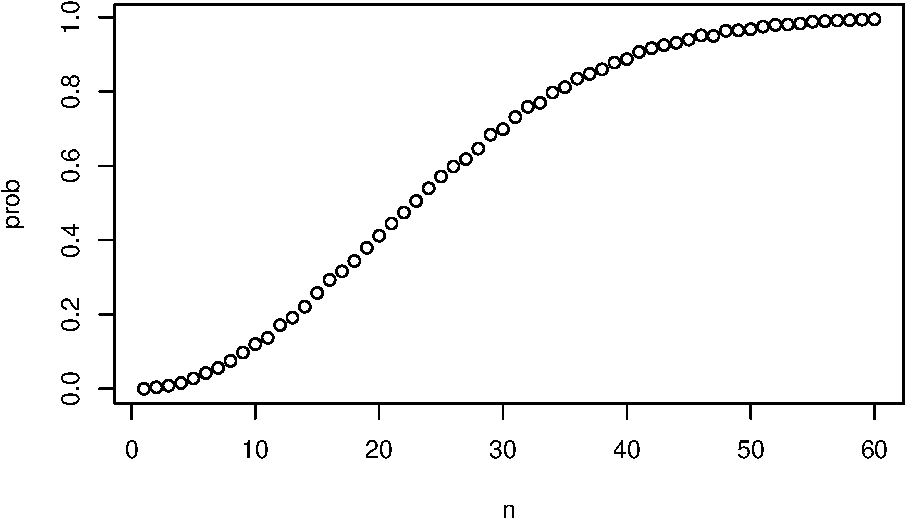
\includegraphics{Data_Science_Probability_files/figure-latex/unnamed-chunk-19-1.pdf}

\emph{Computing birthday problem probabilities with sapply}

\begin{Shaded}
\begin{Highlighting}[]
\CommentTok{\# function for computing exact probability of shared birthdays for any n}
\NormalTok{exact\_prob \textless{}{-}}\StringTok{ }\ControlFlowTok{function}\NormalTok{(n)\{}
\NormalTok{    prob\_unique \textless{}{-}}\StringTok{ }\KeywordTok{seq}\NormalTok{(}\DecValTok{365}\NormalTok{, }\DecValTok{365}\OperatorTok{{-}}\NormalTok{n}\OperatorTok{+}\DecValTok{1}\NormalTok{)}\OperatorTok{/}\DecValTok{365}   \CommentTok{\# vector of fractions for mult. rule}
    \DecValTok{1} \OperatorTok{{-}}\StringTok{ }\KeywordTok{prod}\NormalTok{(prob\_unique)    }\CommentTok{\# calculate prob of no shared birthdays and subtract from 1}
\NormalTok{\}}

\CommentTok{\# applying function element{-}wise to vector of n values}
\NormalTok{eprob \textless{}{-}}\StringTok{ }\KeywordTok{sapply}\NormalTok{(n, exact\_prob)}

\CommentTok{\# plotting Monte Carlo results and exact probabilities on same graph}
\KeywordTok{plot}\NormalTok{(n, prob)    }\CommentTok{\# plot Monte Carlo results}
\KeywordTok{lines}\NormalTok{(n, eprob, }\DataTypeTok{col =} \StringTok{"red"}\NormalTok{)    }\CommentTok{\# add line for exact prob}
\end{Highlighting}
\end{Shaded}

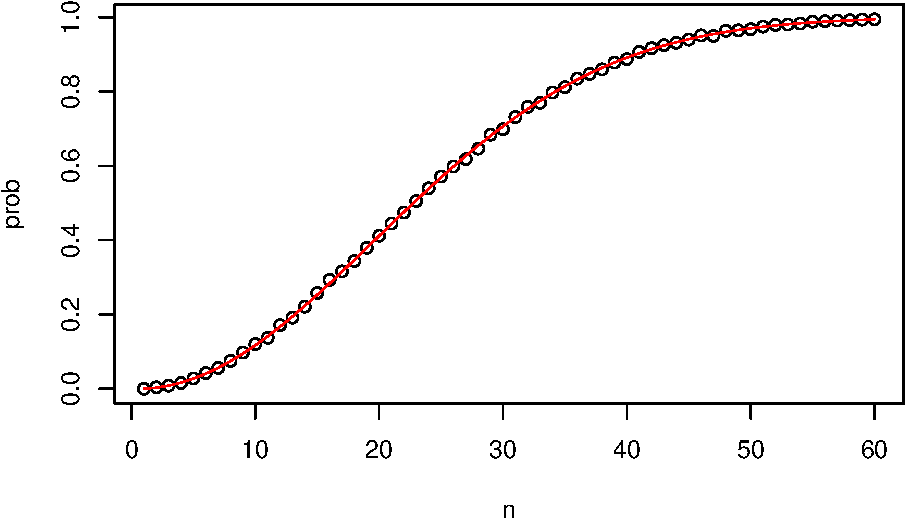
\includegraphics{Data_Science_Probability_files/figure-latex/unnamed-chunk-20-1.pdf}

\hypertarget{how-many-monte-carlo-experiments-are-enough}{%
\subsection{How many Monte Carlo Experiments are
enough?}\label{how-many-monte-carlo-experiments-are-enough}}

Here is a link to the
\href{https://rafalab.github.io/dsbook/probability.html\#infinity-in-practice}{matching
textbook section}.

\textbf{Key points}

\begin{itemize}
\tightlist
\item
  The larger the number of Monte Carlo replicates \(B\), the more
  accurate the estimate.
\item
  Determining the appropriate size for \(B\) can require advanced
  statistics.
\item
  One practical approach is to try many sizes for \(B\) and look for
  sizes that provide stable estimates.
\end{itemize}

\emph{Code: Estimating a practical value of B}

This code runs Monte Carlo simulations to estimate the probability of
shared birthdays using several \textbf{B} values and plots the results.
When \textbf{B} is large enough that the estimated probability stays
stable, then we have selected a useful value of \textbf{B}.

\begin{Shaded}
\begin{Highlighting}[]
\NormalTok{B \textless{}{-}}\StringTok{ }\DecValTok{10}\OperatorTok{\^{}}\KeywordTok{seq}\NormalTok{(}\DecValTok{1}\NormalTok{, }\DecValTok{5}\NormalTok{, }\DataTypeTok{len =} \DecValTok{100}\NormalTok{)    }\CommentTok{\# defines vector of many B values}
\NormalTok{compute\_prob \textless{}{-}}\StringTok{ }\ControlFlowTok{function}\NormalTok{(B, }\DataTypeTok{n =} \DecValTok{22}\NormalTok{)\{    }\CommentTok{\# function to run Monte Carlo simulation with each B}
\NormalTok{    same\_day \textless{}{-}}\StringTok{ }\KeywordTok{replicate}\NormalTok{(B, \{}
\NormalTok{        bdays \textless{}{-}}\StringTok{ }\KeywordTok{sample}\NormalTok{(}\DecValTok{1}\OperatorTok{:}\DecValTok{365}\NormalTok{, n, }\DataTypeTok{replace =} \OtherTok{TRUE}\NormalTok{)}
        \KeywordTok{any}\NormalTok{(}\KeywordTok{duplicated}\NormalTok{(bdays))}
\NormalTok{    \})}
    \KeywordTok{mean}\NormalTok{(same\_day)}
\NormalTok{\}}
\NormalTok{prob \textless{}{-}}\StringTok{ }\KeywordTok{sapply}\NormalTok{(B, compute\_prob)    }\CommentTok{\# apply compute\_prob to many values of B}
\KeywordTok{plot}\NormalTok{(}\KeywordTok{log10}\NormalTok{(B), prob, }\DataTypeTok{type =} \StringTok{"l"}\NormalTok{)    }\CommentTok{\# plot a line graph of estimates}
\end{Highlighting}
\end{Shaded}

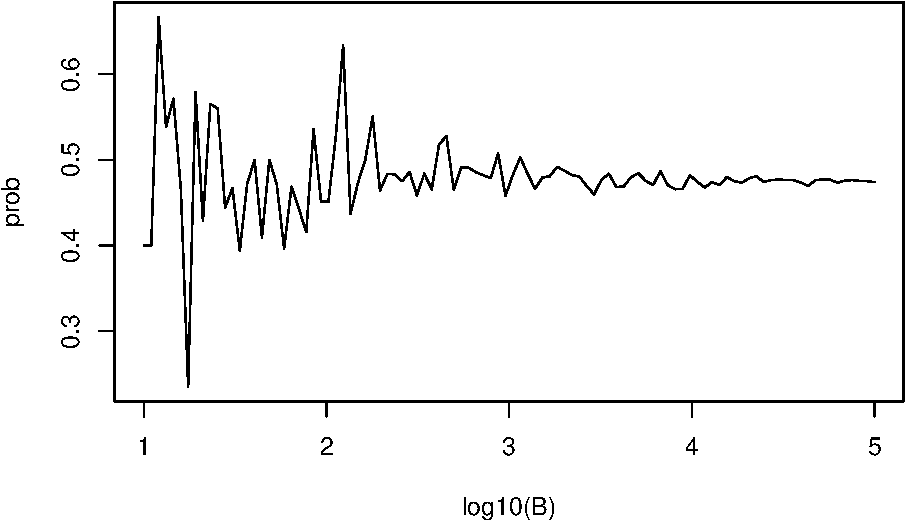
\includegraphics{Data_Science_Probability_files/figure-latex/unnamed-chunk-21-1.pdf}

\hypertarget{assessment---combinations-and-permutations}{%
\subsection{Assessment - Combinations and
Permutations}\label{assessment---combinations-and-permutations}}

1.Imagine you draw two balls from a box containing colored balls. You
either replace the first ball before you draw the second or you leave
the first ball out of the box when you draw the second ball.

Under which situation are the two draws independent of one another?

Remember that two events A and B are independent if:

\(Pr(A\:and\:B) = Pr(A)P(B)\)

\begin{itemize}
\tightlist
\item[$\square$]
  A. You don't replace the first ball before drawing the next.
\item[$\boxtimes$]
  B. You do replace the first ball before drawing the next.
\item[$\square$]
  C. Neither situation describes independent events.
\item[$\square$]
  D. Both situations describe independent events.
\end{itemize}

\begin{enumerate}
\def\labelenumi{\arabic{enumi}.}
\setcounter{enumi}{1}
\tightlist
\item
  Say you've drawn 5 balls from the a box that has 3 cyan balls, 5
  magenta balls, and 7 yellow balls, with replacement, and all have been
  yellow.
\end{enumerate}

What is the probability that the next one is yellow?

\begin{Shaded}
\begin{Highlighting}[]
\CommentTok{\# Assign the variable \textquotesingle{}p\_yellow\textquotesingle{} as the probability that a yellow ball is drawn from the box.}
\NormalTok{p\_yellow \textless{}{-}}\StringTok{ }\NormalTok{yellow }\OperatorTok{/}\StringTok{ }\NormalTok{(cyan }\OperatorTok{+}\StringTok{ }\NormalTok{magenta }\OperatorTok{+}\StringTok{ }\NormalTok{yellow)}

\CommentTok{\# Using the variable \textquotesingle{}p\_yellow\textquotesingle{}, calculate the probability of drawing a yellow ball on the sixth draw. Print this value to the console.}
\NormalTok{p\_yellow}
\end{Highlighting}
\end{Shaded}

\begin{verbatim}
## [1] 0.4666667
\end{verbatim}

\begin{enumerate}
\def\labelenumi{\arabic{enumi}.}
\setcounter{enumi}{2}
\tightlist
\item
  If you roll a 6-sided die once, what is the probability of not seeing
  a 6? If you roll a 6-sided die six times, what is the probability of
  not seeing a 6 on any roll?
\end{enumerate}

\begin{Shaded}
\begin{Highlighting}[]
\CommentTok{\# Assign the variable \textquotesingle{}p\_no6\textquotesingle{} as the probability of not seeing a 6 on a single roll.}
\NormalTok{p\_no6 \textless{}{-}}\StringTok{ }\DecValTok{5}\OperatorTok{/}\DecValTok{6}

\CommentTok{\# Calculate the probability of not seeing a 6 on six rolls using \textasciigrave{}p\_no6\textasciigrave{}. Print your result to the console: do not assign it to a variable.}
\NormalTok{p\_no6}\OperatorTok{*}\NormalTok{p\_no6}\OperatorTok{*}\NormalTok{p\_no6}\OperatorTok{*}\NormalTok{p\_no6}\OperatorTok{*}\NormalTok{p\_no6}\OperatorTok{*}\NormalTok{p\_no6}
\end{Highlighting}
\end{Shaded}

\begin{verbatim}
## [1] 0.334898
\end{verbatim}

\begin{enumerate}
\def\labelenumi{\arabic{enumi}.}
\setcounter{enumi}{3}
\tightlist
\item
  Two teams, say the Celtics and the Cavs, are playing a seven game
  series. The Cavs are a better team and have a 60\% chance of winning
  each game.
\end{enumerate}

What is the probability that the Celtics win at least one game? Remember
that the Celtics must win one of the first four games, or the series
will be over!

\begin{Shaded}
\begin{Highlighting}[]
\CommentTok{\# Assign the variable \textasciigrave{}p\_cavs\_win4\textasciigrave{} as the probability that the Cavs will win the first four games of the series.}
\NormalTok{p\_cavs\_win4 \textless{}{-}}\StringTok{ }\NormalTok{(}\DecValTok{3}\OperatorTok{/}\DecValTok{5}\NormalTok{)}\OperatorTok{*}\NormalTok{(}\DecValTok{3}\OperatorTok{/}\DecValTok{5}\NormalTok{)}\OperatorTok{*}\NormalTok{(}\DecValTok{3}\OperatorTok{/}\DecValTok{5}\NormalTok{)}\OperatorTok{*}\NormalTok{(}\DecValTok{3}\OperatorTok{/}\DecValTok{5}\NormalTok{)}

\CommentTok{\# Using the variable \textasciigrave{}p\_cavs\_win4\textasciigrave{}, calculate the probability that the Celtics win at least one game in the first four games of the series.}
\DecValTok{1}\OperatorTok{{-}}\NormalTok{p\_cavs\_win4}
\end{Highlighting}
\end{Shaded}

\begin{verbatim}
## [1] 0.8704
\end{verbatim}

\begin{enumerate}
\def\labelenumi{\arabic{enumi}.}
\setcounter{enumi}{4}
\tightlist
\item
  Create a Monte Carlo simulation to confirm your answer to the previous
  problem by estimating how frequently the Celtics win at least 1 of 4
  games. Use \texttt{B\ \textless{}-\ 10000} simulations.
\end{enumerate}

The provided sample code simulates a single series of four random games,
\texttt{simulated\_games}

\begin{Shaded}
\begin{Highlighting}[]
\CommentTok{\# This line of example code simulates four independent random games where the Celtics either lose or win. Copy this example code to use within the \textasciigrave{}replicate\textasciigrave{} function.}
\NormalTok{simulated\_games \textless{}{-}}\StringTok{ }\KeywordTok{sample}\NormalTok{(}\KeywordTok{c}\NormalTok{(}\StringTok{"lose"}\NormalTok{,}\StringTok{"win"}\NormalTok{), }\DecValTok{4}\NormalTok{, }\DataTypeTok{replace =} \OtherTok{TRUE}\NormalTok{, }\DataTypeTok{prob =} \KeywordTok{c}\NormalTok{(}\FloatTok{0.6}\NormalTok{, }\FloatTok{0.4}\NormalTok{))}

\CommentTok{\# The variable \textquotesingle{}B\textquotesingle{} specifies the number of times we want the simulation to run. Let\textquotesingle{}s run the Monte Carlo simulation 10,000 times.}
\NormalTok{B \textless{}{-}}\StringTok{ }\DecValTok{10000}

\CommentTok{\# Use the \textasciigrave{}set.seed\textasciigrave{} function to make sure your answer matches the expected result after random sampling.}
\KeywordTok{set.seed}\NormalTok{(}\DecValTok{1}\NormalTok{)}

\CommentTok{\# Create an object called \textasciigrave{}celtic\_wins\textasciigrave{} that replicates two steps for B iterations: (1) generating a random four{-}game series \textasciigrave{}simulated\_games\textasciigrave{} using the example code, then (2) determining whether the simulated series contains at least one win for the Celtics.}
\NormalTok{celtic\_wins \textless{}{-}}\StringTok{ }\KeywordTok{replicate}\NormalTok{(B, \{ }
\NormalTok{  simulated\_games \textless{}{-}}\StringTok{ }\KeywordTok{sample}\NormalTok{(}\KeywordTok{c}\NormalTok{(}\StringTok{"lose"}\NormalTok{,}\StringTok{"win"}\NormalTok{), }\DecValTok{4}\NormalTok{, }\DataTypeTok{replace =} \OtherTok{TRUE}\NormalTok{, }\DataTypeTok{prob =} \KeywordTok{c}\NormalTok{(}\FloatTok{0.6}\NormalTok{, }\FloatTok{0.4}\NormalTok{))}
  \KeywordTok{any}\NormalTok{(simulated\_games}\OperatorTok{==}\StringTok{"win"}\NormalTok{)\}}
\NormalTok{)}

\CommentTok{\# Calculate the frequency out of B iterations that the Celtics won at least one game. Print your answer to the console.}
\KeywordTok{mean}\NormalTok{(celtic\_wins)}
\end{Highlighting}
\end{Shaded}

\begin{verbatim}
## [1] 0.8757
\end{verbatim}

\hypertarget{the-addition-rule}{%
\subsection{The Addition rule}\label{the-addition-rule}}

Here is a link to the textbook section on the
\href{https://rafalab.github.io/dsbook/probability.html\#addition-rule}{addition
rule}.

\textbf{Key points}

\begin{itemize}
\tightlist
\item
  The addition rule states that the probability of event \(A\) or event
  \(B\) happening is the probability of event \(A\) plus the probability
  of event \(B\) minus the probability of both events \(A\) and \(B\)
  happening together.
\end{itemize}

\(Pr(A\:or\:B)=Pr(A) + Pr(B) − Pr(A\:and\:B)\)

Note that \((A\:or\:B)\) is equivalent to \((A \mid B)\).

\emph{Example: The addition rule for a natural 21 in blackjack}

We apply the addition rule where \(A\) = drawing an ace then a facecard
and \(B\) = drawing a facecard then an ace. Note that in this case, both
events A and B cannot happen at the same time, so \(Pr(A\:and\:B) = 0\).

\(Pr(ace\:then\:facecard) = \frac{4}{52}\:X\: \frac{16}{51}\)

\(Pr(facecard\:then\:ace) = \frac{16}{52}\:X\: \frac{4}{51}\)

\(Pr(ace\:then\:facecard \mid facecard\:then\:ace) = \frac{4}{52}\:X\: \frac{16}{51}\:+\:\frac{16}{52}\:X\: \frac{4}{51} = 0.0483\)

\hypertarget{the-monty-hall-problem}{%
\subsection{The Monty Hall Problem}\label{the-monty-hall-problem}}

Here is the textbook section on the
\href{https://rafalab.github.io/dsbook/probability.html\#monty-hall-problem}{Monty
Hall Problem}.

\emph{Key points}

\begin{itemize}
\tightlist
\item
  Monte Carlo simulations can be used to simulate random outcomes, which
  makes them useful when exploring ambiguous or less intuitive problems
  like the Monty Hall problem.
\item
  In the Monty Hall problem, contestants choose one of three doors that
  may contain a prize. Then, one of the doors that was not chosen by the
  contestant and does not contain a prize is revealed. The contestant
  can then choose whether to stick with the original choice or switch to
  the remaining unopened door.
\item
  Although it may seem intuitively like the contestant has a 1 in 2
  chance of winning regardless of whether they stick or switch, Monte
  Carlo simulations demonstrate that the actual probability of winning
  is 1 in 3 with the stick strategy and 2 in 3 with the switch strategy.
\item
  For more on the Monty Hall problem, you can
  \href{https://www.khanacademy.org/math/precalculus/prob-comb/dependent-events-precalc/v/monty-hall-problem}{watch
  a detailed explanation here} or
  \href{https://en.wikipedia.org/wiki/Monty_Hall_problem}{read an
  explanation here}.
\end{itemize}

\emph{Code: Monte Carlo simulation of stick strategy}

\begin{Shaded}
\begin{Highlighting}[]
\NormalTok{B \textless{}{-}}\StringTok{ }\DecValTok{10000}
\NormalTok{stick \textless{}{-}}\StringTok{ }\KeywordTok{replicate}\NormalTok{(B, \{}
\NormalTok{  doors \textless{}{-}}\StringTok{ }\KeywordTok{as.character}\NormalTok{(}\DecValTok{1}\OperatorTok{:}\DecValTok{3}\NormalTok{)}
\NormalTok{  prize \textless{}{-}}\StringTok{ }\KeywordTok{sample}\NormalTok{(}\KeywordTok{c}\NormalTok{(}\StringTok{"car"}\NormalTok{,}\StringTok{"goat"}\NormalTok{,}\StringTok{"goat"}\NormalTok{))    }\CommentTok{\# puts prizes in random order}
\NormalTok{  prize\_door \textless{}{-}}\StringTok{ }\NormalTok{doors[prize }\OperatorTok{==}\StringTok{ "car"}\NormalTok{]    }\CommentTok{\# note which door has prize}
\NormalTok{  my\_pick  \textless{}{-}}\StringTok{ }\KeywordTok{sample}\NormalTok{(doors, }\DecValTok{1}\NormalTok{)    }\CommentTok{\# note which door is chosen}
\NormalTok{  show \textless{}{-}}\StringTok{ }\KeywordTok{sample}\NormalTok{(doors[}\OperatorTok{!}\NormalTok{doors }\OperatorTok{\%in\%}\StringTok{ }\KeywordTok{c}\NormalTok{(my\_pick, prize\_door)],}\DecValTok{1}\NormalTok{)    }\CommentTok{\# open door with no prize that isn\textquotesingle{}t chosen}
\NormalTok{  stick \textless{}{-}}\StringTok{ }\NormalTok{my\_pick    }\CommentTok{\# stick with original door}
\NormalTok{  stick }\OperatorTok{==}\StringTok{ }\NormalTok{prize\_door    }\CommentTok{\# test whether the original door has the prize}
\NormalTok{\})}
\KeywordTok{mean}\NormalTok{(stick)    }\CommentTok{\# probability of choosing prize door when sticking}
\end{Highlighting}
\end{Shaded}

\begin{verbatim}
## [1] 0.3388
\end{verbatim}

\emph{Code: Monte Carlo simulation of switch strategy}

\begin{Shaded}
\begin{Highlighting}[]
\ControlFlowTok{switch}\NormalTok{ \textless{}{-}}\StringTok{ }\KeywordTok{replicate}\NormalTok{(B, \{}
\NormalTok{  doors \textless{}{-}}\StringTok{ }\KeywordTok{as.character}\NormalTok{(}\DecValTok{1}\OperatorTok{:}\DecValTok{3}\NormalTok{)}
\NormalTok{  prize \textless{}{-}}\StringTok{ }\KeywordTok{sample}\NormalTok{(}\KeywordTok{c}\NormalTok{(}\StringTok{"car"}\NormalTok{,}\StringTok{"goat"}\NormalTok{,}\StringTok{"goat"}\NormalTok{))    }\CommentTok{\# puts prizes in random order}
\NormalTok{  prize\_door \textless{}{-}}\StringTok{ }\NormalTok{doors[prize }\OperatorTok{==}\StringTok{ "car"}\NormalTok{]    }\CommentTok{\# note which door has prize}
\NormalTok{  my\_pick  \textless{}{-}}\StringTok{ }\KeywordTok{sample}\NormalTok{(doors, }\DecValTok{1}\NormalTok{)    }\CommentTok{\# note which door is chosen first}
\NormalTok{  show \textless{}{-}}\StringTok{ }\KeywordTok{sample}\NormalTok{(doors[}\OperatorTok{!}\NormalTok{doors }\OperatorTok{\%in\%}\StringTok{ }\KeywordTok{c}\NormalTok{(my\_pick, prize\_door)], }\DecValTok{1}\NormalTok{)    }\CommentTok{\# open door with no prize that isn\textquotesingle{}t chosen}
  \ControlFlowTok{switch}\NormalTok{ \textless{}{-}}\StringTok{ }\NormalTok{doors[}\OperatorTok{!}\NormalTok{doors}\OperatorTok{\%in\%}\KeywordTok{c}\NormalTok{(my\_pick, show)]    }\CommentTok{\# switch to the door that wasn\textquotesingle{}t chosen first or opened}
  \ControlFlowTok{switch} \OperatorTok{==}\StringTok{ }\NormalTok{prize\_door    }\CommentTok{\# test whether the switched door has the prize}
\NormalTok{\})}
\KeywordTok{mean}\NormalTok{(}\ControlFlowTok{switch}\NormalTok{)    }\CommentTok{\# probability of choosing prize door when switching}
\end{Highlighting}
\end{Shaded}

\begin{verbatim}
## [1] 0.6708
\end{verbatim}

\hypertarget{assessment-3-the-addition-rule-and-monty-hall}{%
\subsection{Assessment 3: The Addition Rule and Monty
Hall}\label{assessment-3-the-addition-rule-and-monty-hall}}

\begin{enumerate}
\def\labelenumi{\arabic{enumi}.}
\tightlist
\item
  Two teams, say the Cavs and the Warriors, are playing a seven game
  championship series. The first to win four games wins the series. The
  teams are equally good, so they each have a 50-50 chance of winning
  each game.
\end{enumerate}

If the Cavs lose the first game, what is the probability that they win
the series?

\begin{Shaded}
\begin{Highlighting}[]
\CommentTok{\# Assign a variable \textquotesingle{}n\textquotesingle{} as the number of remaining games.}
\NormalTok{n \textless{}{-}}\DecValTok{6}

\CommentTok{\# Assign a variable \textasciigrave{}outcomes\textasciigrave{} as a vector of possible game outcomes, where 0 indicates a loss and 1 indicates a win for the Cavs.}
\NormalTok{outcomes \textless{}{-}}\StringTok{ }\NormalTok{(}\DecValTok{0}\OperatorTok{:}\DecValTok{1}\NormalTok{)}

\CommentTok{\# Assign a variable \textasciigrave{}l\textasciigrave{} to a list of all possible outcomes in all remaining games. Use the \textasciigrave{}rep\textasciigrave{} function on \textasciigrave{}list(outcomes)\textasciigrave{} to create list of length \textasciigrave{}n\textasciigrave{}.}
\NormalTok{l \textless{}{-}}\StringTok{ }\KeywordTok{rep}\NormalTok{(}\KeywordTok{list}\NormalTok{(outcomes), n)}

\CommentTok{\# Create a data frame named \textquotesingle{}possibilities\textquotesingle{} that contains all combinations of possible outcomes for the remaining games.}
\NormalTok{possibilities \textless{}{-}}\StringTok{ }\KeywordTok{expand.grid}\NormalTok{(l)}

\CommentTok{\# Create a vector named \textquotesingle{}results\textquotesingle{} that indicates whether each row in the data frame \textquotesingle{}possibilities\textquotesingle{} contains enough wins for the Cavs to win the series.}
\NormalTok{results \textless{}{-}}\StringTok{ }\KeywordTok{rowSums}\NormalTok{(possibilities)}\OperatorTok{\textgreater{}=}\DecValTok{4}

\CommentTok{\# Calculate the proportion of \textquotesingle{}results\textquotesingle{} in which the Cavs win the series. Print the outcome to the console.}
\KeywordTok{mean}\NormalTok{(results)}
\end{Highlighting}
\end{Shaded}

\begin{verbatim}
## [1] 0.34375
\end{verbatim}

\begin{enumerate}
\def\labelenumi{\arabic{enumi}.}
\setcounter{enumi}{1}
\tightlist
\item
  Confirm the results of the previous question with a Monte Carlo
  simulation to estimate the probability of the Cavs winning the series
  after losing the first game.
\end{enumerate}

\begin{Shaded}
\begin{Highlighting}[]
\CommentTok{\# The variable \textasciigrave{}B\textasciigrave{} specifies the number of times we want the simulation to run. Let\textquotesingle{}s run the Monte Carlo simulation 10,000 times.}
\NormalTok{B \textless{}{-}}\StringTok{ }\DecValTok{10000}

\CommentTok{\# Use the \textasciigrave{}set.seed\textasciigrave{} function to make sure your answer matches the expected result after random sampling.}
\KeywordTok{set.seed}\NormalTok{(}\DecValTok{1}\NormalTok{)}

\CommentTok{\# Create an object called \textasciigrave{}results\textasciigrave{} that replicates for \textasciigrave{}B\textasciigrave{} iterations a simulated series and determines whether that series contains at least four wins for the Cavs.}
\NormalTok{results \textless{}{-}}\StringTok{ }\KeywordTok{replicate}\NormalTok{(B, \{ }
\NormalTok{  cavs\_wins \textless{}{-}}\StringTok{ }\KeywordTok{sample}\NormalTok{(}\KeywordTok{c}\NormalTok{(}\DecValTok{0}\NormalTok{,}\DecValTok{1}\NormalTok{), }\DecValTok{6}\NormalTok{, }\DataTypeTok{replace =} \OtherTok{TRUE}\NormalTok{)}
  \KeywordTok{sum}\NormalTok{(cavs\_wins)}\OperatorTok{\textgreater{}=}\DecValTok{4}\NormalTok{ \}}
\NormalTok{)}

\CommentTok{\# Calculate the frequency out of \textasciigrave{}B\textasciigrave{} iterations that the Cavs won at least four games in the remainder of the series. Print your answer to the console.}
\KeywordTok{mean}\NormalTok{(results)}
\end{Highlighting}
\end{Shaded}

\begin{verbatim}
## [1] 0.3371
\end{verbatim}

\begin{enumerate}
\def\labelenumi{\arabic{enumi}.}
\setcounter{enumi}{2}
\tightlist
\item
  Two teams, \(A\) and \(B\), are playing a seven series game series.
  Team \(A\) is better than team \(B\) and has a
  \texttt{p\ \textgreater{}\ 0.5} chance of winning each game.
\end{enumerate}

\begin{Shaded}
\begin{Highlighting}[]
\CommentTok{\# Let\textquotesingle{}s assign the variable \textquotesingle{}p\textquotesingle{} as the vector of probabilities that team A will win.}
\NormalTok{p \textless{}{-}}\StringTok{ }\KeywordTok{seq}\NormalTok{(}\FloatTok{0.5}\NormalTok{, }\FloatTok{0.95}\NormalTok{, }\FloatTok{0.025}\NormalTok{)}

\CommentTok{\# Given a value \textquotesingle{}p\textquotesingle{}, the probability of winning the series for the underdog team B can be computed with the following function based on a Monte Carlo simulation:}
\NormalTok{prob\_win \textless{}{-}}\StringTok{ }\ControlFlowTok{function}\NormalTok{(p)\{}
\NormalTok{  B \textless{}{-}}\StringTok{ }\DecValTok{10000}
\NormalTok{  result \textless{}{-}}\StringTok{ }\KeywordTok{replicate}\NormalTok{(B, \{}
\NormalTok{    b\_win \textless{}{-}}\StringTok{ }\KeywordTok{sample}\NormalTok{(}\KeywordTok{c}\NormalTok{(}\DecValTok{1}\NormalTok{,}\DecValTok{0}\NormalTok{), }\DecValTok{7}\NormalTok{, }\DataTypeTok{replace =} \OtherTok{TRUE}\NormalTok{, }\DataTypeTok{prob =} \KeywordTok{c}\NormalTok{(}\DecValTok{1}\OperatorTok{{-}}\NormalTok{p, p))}
    \KeywordTok{sum}\NormalTok{(b\_win)}\OperatorTok{\textgreater{}=}\DecValTok{4}
\NormalTok{    \})}
  \KeywordTok{mean}\NormalTok{(result)}
\NormalTok{\}}

\CommentTok{\# Apply the \textquotesingle{}prob\_win\textquotesingle{} function across the vector of probabilities that team A will win to determine the probability that team B will win. Call this object \textquotesingle{}Pr\textquotesingle{}.}
\NormalTok{Pr \textless{}{-}}\StringTok{ }\KeywordTok{sapply}\NormalTok{(p, prob\_win)}

\CommentTok{\# Plot the probability \textquotesingle{}p\textquotesingle{} on the x{-}axis and \textquotesingle{}Pr\textquotesingle{} on the y{-}axis.}
\KeywordTok{plot}\NormalTok{(p,Pr)}
\end{Highlighting}
\end{Shaded}

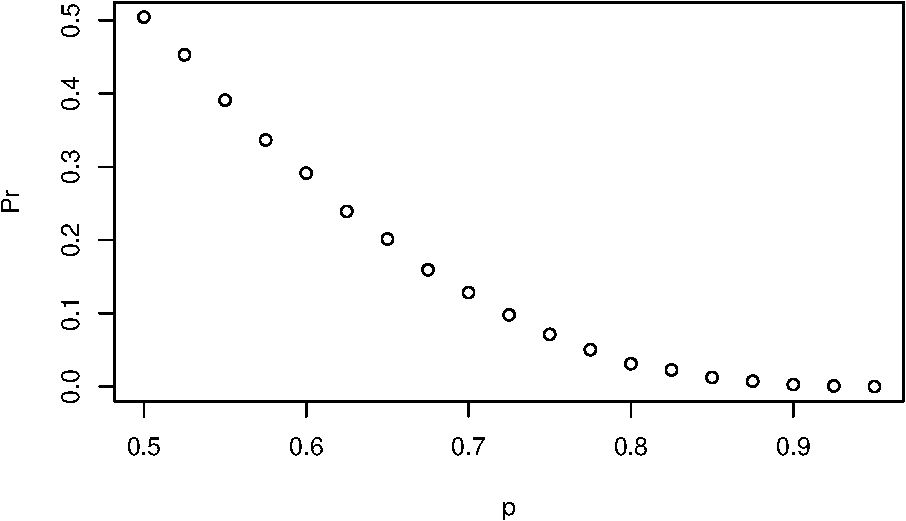
\includegraphics{Data_Science_Probability_files/figure-latex/unnamed-chunk-30-1.pdf}

\begin{enumerate}
\def\labelenumi{\arabic{enumi}.}
\setcounter{enumi}{3}
\tightlist
\item
  Repeat the previous exercise, but now keep the probability that team
  \(A\) wins fixed at \texttt{p\ \textless{}-\ 0.75} and compute the
  probability for different series lengths.
\end{enumerate}

For example, wins in best of 1 game, 3 games, 5 games, and so on through
a series that lasts 25 games.

\begin{Shaded}
\begin{Highlighting}[]
\CommentTok{\# Given a value \textquotesingle{}p\textquotesingle{}, the probability of winning the series for the underdog team B can be computed with the following function based on a Monte Carlo simulation:}
\NormalTok{prob\_win \textless{}{-}}\StringTok{ }\ControlFlowTok{function}\NormalTok{(N, }\DataTypeTok{p=}\FloatTok{0.75}\NormalTok{)\{}
\NormalTok{      B \textless{}{-}}\StringTok{ }\DecValTok{10000}
\NormalTok{      result \textless{}{-}}\StringTok{ }\KeywordTok{replicate}\NormalTok{(B, \{}
\NormalTok{        b\_win \textless{}{-}}\StringTok{ }\KeywordTok{sample}\NormalTok{(}\KeywordTok{c}\NormalTok{(}\DecValTok{1}\NormalTok{,}\DecValTok{0}\NormalTok{), N, }\DataTypeTok{replace =} \OtherTok{TRUE}\NormalTok{, }\DataTypeTok{prob =} \KeywordTok{c}\NormalTok{(}\DecValTok{1}\OperatorTok{{-}}\NormalTok{p, p))}
        \KeywordTok{sum}\NormalTok{(b\_win)}\OperatorTok{\textgreater{}=}\NormalTok{(N}\OperatorTok{+}\DecValTok{1}\NormalTok{)}\OperatorTok{/}\DecValTok{2}
\NormalTok{        \})}
      \KeywordTok{mean}\NormalTok{(result)}
\NormalTok{    \}}

\CommentTok{\# Assign the variable \textquotesingle{}N\textquotesingle{} as the vector of series lengths. Use only odd numbers ranging from 1 to 25 games.}
\NormalTok{N \textless{}{-}}\StringTok{ }\KeywordTok{seq}\NormalTok{(}\DecValTok{1}\NormalTok{, }\DecValTok{25}\NormalTok{, }\DecValTok{2}\NormalTok{)}

\CommentTok{\# Apply the \textquotesingle{}prob\_win\textquotesingle{} function across the vector of series lengths to determine the probability that team B will win. Call this object \textasciigrave{}Pr\textasciigrave{}.}
\NormalTok{Pr \textless{}{-}}\StringTok{ }\KeywordTok{sapply}\NormalTok{(N, prob\_win)}

\CommentTok{\# Plot the number of games in the series \textquotesingle{}N\textquotesingle{} on the x{-}axis and \textquotesingle{}Pr\textquotesingle{} on the y{-}axis.}
\KeywordTok{plot}\NormalTok{(N,Pr)}
\end{Highlighting}
\end{Shaded}

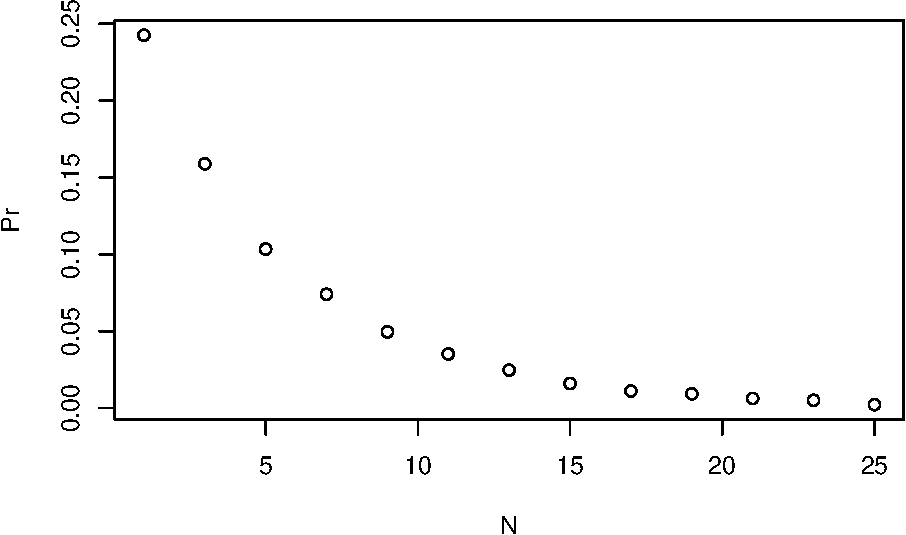
\includegraphics{Data_Science_Probability_files/figure-latex/unnamed-chunk-31-1.pdf}

\hypertarget{assessment---olympic-running}{%
\subsection{Assessment - Olympic
Running}\label{assessment---olympic-running}}

\begin{Shaded}
\begin{Highlighting}[]
\ControlFlowTok{if}\NormalTok{(}\OperatorTok{!}\KeywordTok{require}\NormalTok{(tidyverse)) }\KeywordTok{install.packages}\NormalTok{(}\StringTok{"tidyverse"}\NormalTok{)}
\end{Highlighting}
\end{Shaded}

\begin{verbatim}
## Loading required package: tidyverse
\end{verbatim}

\begin{verbatim}
## -- Attaching packages --------------------------------------------------------------------------------------------------------------------------------------------- tidyverse 1.3.0 --
\end{verbatim}

\begin{verbatim}
## v ggplot2 3.3.2     v purrr   0.3.4
## v tibble  3.0.3     v dplyr   1.0.1
## v tidyr   1.1.1     v stringr 1.4.0
## v readr   1.3.1     v forcats 0.5.0
\end{verbatim}

\begin{verbatim}
## -- Conflicts ------------------------------------------------------------------------------------------------------------------------------------------------ tidyverse_conflicts() --
## x dplyr::filter() masks stats::filter()
## x dplyr::lag()    masks stats::lag()
\end{verbatim}

\begin{Shaded}
\begin{Highlighting}[]
\KeywordTok{library}\NormalTok{(tidyverse)}
\KeywordTok{options}\NormalTok{(}\DataTypeTok{digits =} \DecValTok{3}\NormalTok{)    }\CommentTok{\# report 3 significant digits}
\end{Highlighting}
\end{Shaded}

\begin{enumerate}
\def\labelenumi{\arabic{enumi}.}
\tightlist
\item
  In the 200m dash finals in the Olympics, 8 runners compete for 3
  medals (order matters). In the 2012 Olympics, 3 of the 8 runners were
  from Jamaica and the other 5 were from different countries. The three
  medals were all won by Jamaica (Usain Bolt, Yohan Blake, and Warren
  Weir).
\end{enumerate}

Use the information above to help you answer the following four
questions.

1a. How many different ways can the 3 medals be distributed across 8
runners?

\begin{Shaded}
\begin{Highlighting}[]
\NormalTok{medals \textless{}{-}}\StringTok{ }\KeywordTok{permutations}\NormalTok{(}\DecValTok{8}\NormalTok{,}\DecValTok{3}\NormalTok{)}
\KeywordTok{nrow}\NormalTok{(medals)}
\end{Highlighting}
\end{Shaded}

\begin{verbatim}
## [1] 336
\end{verbatim}

1b. How many different ways can the three medals be distributed among
the 3 runners from Jamaica?

\begin{Shaded}
\begin{Highlighting}[]
\NormalTok{jamaica \textless{}{-}}\StringTok{ }\KeywordTok{permutations}\NormalTok{(}\DecValTok{3}\NormalTok{,}\DecValTok{3}\NormalTok{)}
\KeywordTok{nrow}\NormalTok{(jamaica)}
\end{Highlighting}
\end{Shaded}

\begin{verbatim}
## [1] 6
\end{verbatim}

1c. What is the probability that all 3 medals are won by Jamaica?

\begin{Shaded}
\begin{Highlighting}[]
\KeywordTok{nrow}\NormalTok{(jamaica)}\OperatorTok{/}\KeywordTok{nrow}\NormalTok{(medals)}
\end{Highlighting}
\end{Shaded}

\begin{verbatim}
## [1] 0.0179
\end{verbatim}

1d. Run a Monte Carlo simulation on this vector representing the
countries of the 8 runners in this race:

\begin{Shaded}
\begin{Highlighting}[]
\NormalTok{runners \textless{}{-}}\StringTok{ }\KeywordTok{c}\NormalTok{(}\StringTok{"Jamaica"}\NormalTok{, }\StringTok{"Jamaica"}\NormalTok{, }\StringTok{"Jamaica"}\NormalTok{, }\StringTok{"USA"}\NormalTok{, }\StringTok{"Ecuador"}\NormalTok{, }\StringTok{"Netherlands"}\NormalTok{, }\StringTok{"France"}\NormalTok{, }\StringTok{"South Africa"}\NormalTok{)}
\end{Highlighting}
\end{Shaded}

For each iteration of the Monte Carlo simulation, within a
\texttt{replicate} loop, select 3 runners representing the 3 medalists
and check whether they are all from Jamaica. Repeat this simulation
10,000 times. Set the seed to 1 before running the loop.

Calculate the probability that all the runners are from Jamaica.

\begin{Shaded}
\begin{Highlighting}[]
\KeywordTok{set.seed}\NormalTok{(}\DecValTok{1}\NormalTok{)}
\NormalTok{runners \textless{}{-}}\StringTok{ }\KeywordTok{c}\NormalTok{(}\StringTok{"Jamaica"}\NormalTok{, }\StringTok{"Jamaica"}\NormalTok{, }\StringTok{"Jamaica"}\NormalTok{, }\StringTok{"USA"}\NormalTok{, }\StringTok{"Ecuador"}\NormalTok{, }\StringTok{"Netherlands"}\NormalTok{, }\StringTok{"France"}\NormalTok{, }\StringTok{"South Africa"}\NormalTok{)}
\NormalTok{B \textless{}{-}}\StringTok{ }\DecValTok{10000}
\NormalTok{all\_jamaica \textless{}{-}}\StringTok{ }\KeywordTok{replicate}\NormalTok{(B, \{}
\NormalTok{  results \textless{}{-}}\StringTok{ }\KeywordTok{sample}\NormalTok{(runners, }\DecValTok{3}\NormalTok{)}
  \KeywordTok{all}\NormalTok{(results }\OperatorTok{==}\StringTok{ "Jamaica"}\NormalTok{)}
\NormalTok{\})}
\KeywordTok{mean}\NormalTok{(all\_jamaica)}
\end{Highlighting}
\end{Shaded}

\begin{verbatim}
## [1] 0.0174
\end{verbatim}

\hypertarget{assessment---restaurant-management}{%
\subsection{Assessment - Restaurant
Management}\label{assessment---restaurant-management}}

2: Use the information below to answer the following five questions.

A restaurant manager wants to advertise that his lunch special offers
enough choices to eat different meals every day of the year. He doesn't
think his current special actually allows that number of choices, but
wants to change his special if needed to allow at least 365 choices.

A meal at the restaurant includes 1 entree, 2 sides, and 1 drink. He
currently offers a choice of 1 entree from a list of 6 options, a choice
of 2 different sides from a list of 6 options, and a choice of 1 drink
from a list of 2 options.

2a. How many meal combinations are possible with the current menu?

\begin{Shaded}
\begin{Highlighting}[]
\DecValTok{6} \OperatorTok{*}\StringTok{ }\KeywordTok{nrow}\NormalTok{(}\KeywordTok{combinations}\NormalTok{(}\DecValTok{6}\NormalTok{,}\DecValTok{2}\NormalTok{)) }\OperatorTok{*}\StringTok{ }\DecValTok{2}
\end{Highlighting}
\end{Shaded}

\begin{verbatim}
## [1] 180
\end{verbatim}

2b. The manager has one additional drink he could add to the special.

How many combinations are possible if he expands his original special to
3 drink options?

\begin{Shaded}
\begin{Highlighting}[]
\DecValTok{6} \OperatorTok{*}\StringTok{ }\KeywordTok{nrow}\NormalTok{(}\KeywordTok{combinations}\NormalTok{(}\DecValTok{6}\NormalTok{,}\DecValTok{2}\NormalTok{)) }\OperatorTok{*}\StringTok{ }\DecValTok{3}
\end{Highlighting}
\end{Shaded}

\begin{verbatim}
## [1] 270
\end{verbatim}

2c. The manager decides to add the third drink but needs to expand the
number of options. The manager would prefer not to change his menu
further and wants to know if he can meet his goal by letting customers
choose more sides.

How many meal combinations are there if customers can choose from 6
entrees, 3 drinks, and select 3 sides from the current 6 options?

\begin{Shaded}
\begin{Highlighting}[]
\DecValTok{6} \OperatorTok{*}\StringTok{ }\KeywordTok{nrow}\NormalTok{(}\KeywordTok{combinations}\NormalTok{(}\DecValTok{6}\NormalTok{,}\DecValTok{3}\NormalTok{)) }\OperatorTok{*}\StringTok{ }\DecValTok{3}
\end{Highlighting}
\end{Shaded}

\begin{verbatim}
## [1] 360
\end{verbatim}

2d. The manager is concerned that customers may not want 3 sides with
their meal. He is willing to increase the number of entree choices
instead, but if he adds too many expensive options it could eat into
profits. He wants to know how many entree choices he would have to offer
in order to meet his goal.

\begin{itemize}
\tightlist
\item
  Write a function that takes a number of entree choices and returns the
  number of meal combinations possible given that number of entree
  options, 3 drink choices, and a selection of 2 sides from 6 options.
\item
  Use \texttt{sapply} to apply the function to entree option counts
  ranging from 1 to 12.
\end{itemize}

What is the minimum number of entree options required in order to
generate more than 365 combinations?

\begin{Shaded}
\begin{Highlighting}[]
\NormalTok{entree\_choices \textless{}{-}}\StringTok{ }\ControlFlowTok{function}\NormalTok{(x)\{}
\NormalTok{  x }\OperatorTok{*}\StringTok{ }\KeywordTok{nrow}\NormalTok{(}\KeywordTok{combinations}\NormalTok{(}\DecValTok{6}\NormalTok{,}\DecValTok{2}\NormalTok{)) }\OperatorTok{*}\StringTok{ }\DecValTok{3}
\NormalTok{\}}

\NormalTok{combos \textless{}{-}}\StringTok{ }\KeywordTok{sapply}\NormalTok{(}\DecValTok{1}\OperatorTok{:}\DecValTok{12}\NormalTok{, entree\_choices)}

\KeywordTok{data.frame}\NormalTok{(}\DataTypeTok{entrees =} \DecValTok{1}\OperatorTok{:}\DecValTok{12}\NormalTok{, }\DataTypeTok{combos =}\NormalTok{ combos) }\OperatorTok{\%\textgreater{}\%}
\StringTok{  }\KeywordTok{filter}\NormalTok{(combos }\OperatorTok{\textgreater{}}\StringTok{ }\DecValTok{365}\NormalTok{) }\OperatorTok{\%\textgreater{}\%}
\StringTok{  }\KeywordTok{min}\NormalTok{(.}\OperatorTok{$}\NormalTok{entrees)}
\end{Highlighting}
\end{Shaded}

\begin{verbatim}
## [1] 9
\end{verbatim}

2e. The manager isn't sure he can afford to put that many entree choices
on the lunch menu and thinks it would be cheaper for him to expand the
number of sides. He wants to know how many sides he would have to offer
to meet his goal of at least 365 combinations.

\begin{itemize}
\tightlist
\item
  Write a function that takes a number of side choices and returns the
  number of meal combinations possible given 6 entree choices, 3 drink
  choices, and a selection of 2 sides from the specified number of side
  choices.
\item
  Use \texttt{sapply} to apply the function to side counts ranging from
  2 to 12.
\end{itemize}

What is the minimum number of side options required in order to generate
more than 365 combinations?

\begin{Shaded}
\begin{Highlighting}[]
\NormalTok{side\_choices \textless{}{-}}\StringTok{ }\ControlFlowTok{function}\NormalTok{(x)\{}
  \DecValTok{6} \OperatorTok{*}\StringTok{ }\KeywordTok{nrow}\NormalTok{(}\KeywordTok{combinations}\NormalTok{(x, }\DecValTok{2}\NormalTok{)) }\OperatorTok{*}\StringTok{ }\DecValTok{3}
\NormalTok{\}}

\NormalTok{combos \textless{}{-}}\StringTok{ }\KeywordTok{sapply}\NormalTok{(}\DecValTok{2}\OperatorTok{:}\DecValTok{12}\NormalTok{, side\_choices)}

\KeywordTok{data.frame}\NormalTok{(}\DataTypeTok{sides =} \DecValTok{2}\OperatorTok{:}\DecValTok{12}\NormalTok{, }\DataTypeTok{combos =}\NormalTok{ combos) }\OperatorTok{\%\textgreater{}\%}
\StringTok{  }\KeywordTok{filter}\NormalTok{(combos }\OperatorTok{\textgreater{}}\StringTok{ }\DecValTok{365}\NormalTok{) }\OperatorTok{\%\textgreater{}\%}
\StringTok{  }\KeywordTok{min}\NormalTok{(.}\OperatorTok{$}\NormalTok{sides)}
\end{Highlighting}
\end{Shaded}

\begin{verbatim}
## [1] 7
\end{verbatim}

\hypertarget{assessment---esophageal-cancer-and-alcoholtobacco-use}{%
\subsection{Assessment - Esophageal cancer and alcohol/tobacco
use}\label{assessment---esophageal-cancer-and-alcoholtobacco-use}}

3., 4., 5. and 6. Case-control studies help determine whether certain
exposures are associated with outcomes such as developing cancer. The
built-in dataset \textbf{esoph} contains data from a case-control study
in France comparing people with esophageal cancer (cases, counted in
\textbf{ncases}) to people without esophageal cancer (controls, counted
in \textbf{ncontrols}) that are carefully matched on a variety of
demographic and medical characteristics. The study compares alcohol
intake in grams per day (\textbf{alcgp}) and tobacco intake in grams per
day (\textbf{tobgp}) across cases and controls grouped by age range
(\textbf{agegp}).

The dataset is available in base R and can be called with the variable
name \textbf{esoph}:

\begin{Shaded}
\begin{Highlighting}[]
\KeywordTok{head}\NormalTok{(esoph)}
\end{Highlighting}
\end{Shaded}

\begin{verbatim}
##   agegp     alcgp    tobgp ncases ncontrols
## 1 25-34 0-39g/day 0-9g/day      0        40
## 2 25-34 0-39g/day    10-19      0        10
## 3 25-34 0-39g/day    20-29      0         6
## 4 25-34 0-39g/day      30+      0         5
## 5 25-34     40-79 0-9g/day      0        27
## 6 25-34     40-79    10-19      0         7
\end{verbatim}

You will be using this dataset to answer the following four multi-part
questions (Questions 3-6).

You may wish to use the tidyverse package.

The following three parts have you explore some basic characteristics of
the dataset.

Each row contains one group of the experiment. Each group has a
different combination of age, alcohol consumption, and tobacco
consumption. The number of cancer cases and number of controls
(individuals without cancer) are reported for each group.

3a. How many groups are in the study?

\begin{Shaded}
\begin{Highlighting}[]
\KeywordTok{nrow}\NormalTok{(esoph)}
\end{Highlighting}
\end{Shaded}

\begin{verbatim}
## [1] 88
\end{verbatim}

3b. How many cases are there?

Save this value as \texttt{all\_cases} for later problems.

\begin{Shaded}
\begin{Highlighting}[]
\NormalTok{all\_cases \textless{}{-}}\StringTok{ }\KeywordTok{sum}\NormalTok{(esoph}\OperatorTok{$}\NormalTok{ncases)}
\NormalTok{all\_cases}
\end{Highlighting}
\end{Shaded}

\begin{verbatim}
## [1] 200
\end{verbatim}

3c. How many controls are there?

Save this value as \texttt{all\_controls} for later problems. Remember
from the instructions that controls are individuals without cancer.

\begin{Shaded}
\begin{Highlighting}[]
\NormalTok{all\_controls \textless{}{-}}\StringTok{ }\KeywordTok{sum}\NormalTok{(esoph}\OperatorTok{$}\NormalTok{ncontrols)}
\NormalTok{all\_controls}
\end{Highlighting}
\end{Shaded}

\begin{verbatim}
## [1] 975
\end{verbatim}

4a. What is the probability that a subject in the highest alcohol
consumption group is a cancer case?

Remember that the total number of individuals in the study includes
people with cancer (cases) and people without cancer (controls), so you
must add both values together to get the denominator for your
probability.

\begin{Shaded}
\begin{Highlighting}[]
\NormalTok{esoph }\OperatorTok{\%\textgreater{}\%}
\StringTok{  }\KeywordTok{filter}\NormalTok{(alcgp }\OperatorTok{==}\StringTok{ "120+"}\NormalTok{) }\OperatorTok{\%\textgreater{}\%}
\StringTok{  }\KeywordTok{summarize}\NormalTok{(}\DataTypeTok{ncases =} \KeywordTok{sum}\NormalTok{(ncases), }\DataTypeTok{ncontrols =} \KeywordTok{sum}\NormalTok{(ncontrols)) }\OperatorTok{\%\textgreater{}\%}
\StringTok{  }\KeywordTok{mutate}\NormalTok{(}\DataTypeTok{p\_case =}\NormalTok{ ncases }\OperatorTok{/}\StringTok{ }\NormalTok{(ncases }\OperatorTok{+}\StringTok{ }\NormalTok{ncontrols)) }\OperatorTok{\%\textgreater{}\%}
\StringTok{  }\KeywordTok{pull}\NormalTok{(p\_case)}
\end{Highlighting}
\end{Shaded}

\begin{verbatim}
## [1] 0.402
\end{verbatim}

4b. What is the probability that a subject in the lowest alcohol
consumption group is a cancer case?

\begin{Shaded}
\begin{Highlighting}[]
\NormalTok{esoph }\OperatorTok{\%\textgreater{}\%}
\StringTok{  }\KeywordTok{filter}\NormalTok{(alcgp }\OperatorTok{==}\StringTok{ "0{-}39g/day"}\NormalTok{) }\OperatorTok{\%\textgreater{}\%}
\StringTok{  }\KeywordTok{summarize}\NormalTok{(}\DataTypeTok{ncases =} \KeywordTok{sum}\NormalTok{(ncases), }\DataTypeTok{ncontrols =} \KeywordTok{sum}\NormalTok{(ncontrols)) }\OperatorTok{\%\textgreater{}\%}
\StringTok{  }\KeywordTok{mutate}\NormalTok{(}\DataTypeTok{p\_case =}\NormalTok{ ncases }\OperatorTok{/}\StringTok{ }\NormalTok{(ncases }\OperatorTok{+}\StringTok{ }\NormalTok{ncontrols)) }\OperatorTok{\%\textgreater{}\%}
\StringTok{  }\KeywordTok{pull}\NormalTok{(p\_case)}
\end{Highlighting}
\end{Shaded}

\begin{verbatim}
## [1] 0.0653
\end{verbatim}

4c. Given that a person is a case, what is the probability that they
smoke 10g or more a day?

\begin{Shaded}
\begin{Highlighting}[]
\NormalTok{tob\_cases \textless{}{-}}\StringTok{ }\NormalTok{esoph }\OperatorTok{\%\textgreater{}\%}
\StringTok{  }\KeywordTok{filter}\NormalTok{(tobgp }\OperatorTok{!=}\StringTok{ "0{-}9g/day"}\NormalTok{) }\OperatorTok{\%\textgreater{}\%}
\StringTok{  }\KeywordTok{pull}\NormalTok{(ncases) }\OperatorTok{\%\textgreater{}\%}
\StringTok{  }\KeywordTok{sum}\NormalTok{()}

\NormalTok{tob\_cases}\OperatorTok{/}\NormalTok{all\_cases}
\end{Highlighting}
\end{Shaded}

\begin{verbatim}
## [1] 0.61
\end{verbatim}

4d. Given that a person is a control, what is the probability that they
smoke 10g or more a day?

\begin{Shaded}
\begin{Highlighting}[]
\NormalTok{tob\_controls \textless{}{-}}\StringTok{ }\NormalTok{esoph }\OperatorTok{\%\textgreater{}\%}
\StringTok{  }\KeywordTok{filter}\NormalTok{(tobgp }\OperatorTok{!=}\StringTok{ "0{-}9g/day"}\NormalTok{) }\OperatorTok{\%\textgreater{}\%}
\StringTok{  }\KeywordTok{pull}\NormalTok{(ncontrols) }\OperatorTok{\%\textgreater{}\%}
\StringTok{  }\KeywordTok{sum}\NormalTok{()}

\NormalTok{tob\_controls}\OperatorTok{/}\NormalTok{all\_controls}
\end{Highlighting}
\end{Shaded}

\begin{verbatim}
## [1] 0.462
\end{verbatim}

5a. For cases, what is the probability of being in the highest alcohol
group?

\begin{Shaded}
\begin{Highlighting}[]
\NormalTok{high\_alc\_cases \textless{}{-}}\StringTok{ }\NormalTok{esoph }\OperatorTok{\%\textgreater{}\%}
\StringTok{  }\KeywordTok{filter}\NormalTok{(alcgp }\OperatorTok{==}\StringTok{ "120+"}\NormalTok{) }\OperatorTok{\%\textgreater{}\%}
\StringTok{  }\KeywordTok{pull}\NormalTok{(ncases) }\OperatorTok{\%\textgreater{}\%}
\StringTok{  }\KeywordTok{sum}\NormalTok{()}

\NormalTok{p\_case\_high\_alc \textless{}{-}}\StringTok{ }\NormalTok{high\_alc\_cases}\OperatorTok{/}\NormalTok{all\_cases}
\NormalTok{p\_case\_high\_alc}
\end{Highlighting}
\end{Shaded}

\begin{verbatim}
## [1] 0.225
\end{verbatim}

5b. For cases, what is the probability of being in the highest tobacco
group?

\begin{Shaded}
\begin{Highlighting}[]
\NormalTok{high\_tob\_cases \textless{}{-}}\StringTok{ }\NormalTok{esoph }\OperatorTok{\%\textgreater{}\%}
\StringTok{  }\KeywordTok{filter}\NormalTok{(tobgp }\OperatorTok{==}\StringTok{ "30+"}\NormalTok{) }\OperatorTok{\%\textgreater{}\%}
\StringTok{  }\KeywordTok{pull}\NormalTok{(ncases) }\OperatorTok{\%\textgreater{}\%}
\StringTok{  }\KeywordTok{sum}\NormalTok{()}

\NormalTok{p\_case\_high\_tob \textless{}{-}}\StringTok{ }\NormalTok{high\_tob\_cases}\OperatorTok{/}\NormalTok{all\_cases}
\NormalTok{p\_case\_high\_tob}
\end{Highlighting}
\end{Shaded}

\begin{verbatim}
## [1] 0.155
\end{verbatim}

5c. For cases, what is the probability of being in the highest alcohol
group \textbf{and} the highest tobacco group?

\begin{Shaded}
\begin{Highlighting}[]
\NormalTok{high\_alc\_tob\_cases \textless{}{-}}\StringTok{ }\NormalTok{esoph }\OperatorTok{\%\textgreater{}\%}
\StringTok{  }\KeywordTok{filter}\NormalTok{(alcgp }\OperatorTok{==}\StringTok{ "120+"} \OperatorTok{\&}\StringTok{ }\NormalTok{tobgp }\OperatorTok{==}\StringTok{ "30+"}\NormalTok{) }\OperatorTok{\%\textgreater{}\%}
\StringTok{  }\KeywordTok{pull}\NormalTok{(ncases) }\OperatorTok{\%\textgreater{}\%}
\StringTok{  }\KeywordTok{sum}\NormalTok{()}

\NormalTok{p\_case\_high\_alc\_tob \textless{}{-}}\StringTok{ }\NormalTok{high\_alc\_tob\_cases}\OperatorTok{/}\NormalTok{all\_cases}
\NormalTok{p\_case\_high\_alc\_tob}
\end{Highlighting}
\end{Shaded}

\begin{verbatim}
## [1] 0.05
\end{verbatim}

5d. For cases, what is the probability of being in the highest alcohol
group \textbf{or} the highest tobacco group?

\begin{Shaded}
\begin{Highlighting}[]
\NormalTok{p\_case\_either\_highest \textless{}{-}}\StringTok{ }\NormalTok{p\_case\_high\_alc }\OperatorTok{+}\StringTok{ }\NormalTok{p\_case\_high\_tob }\OperatorTok{{-}}\StringTok{ }\NormalTok{p\_case\_high\_alc\_tob}
\NormalTok{p\_case\_either\_highest}
\end{Highlighting}
\end{Shaded}

\begin{verbatim}
## [1] 0.33
\end{verbatim}

6a. For controls, what is the probability of being in the highest
alcohol group?

\begin{Shaded}
\begin{Highlighting}[]
\NormalTok{high\_alc\_controls \textless{}{-}}\StringTok{ }\NormalTok{esoph }\OperatorTok{\%\textgreater{}\%}
\StringTok{  }\KeywordTok{filter}\NormalTok{(alcgp }\OperatorTok{==}\StringTok{ "120+"}\NormalTok{) }\OperatorTok{\%\textgreater{}\%}
\StringTok{  }\KeywordTok{pull}\NormalTok{(ncontrols) }\OperatorTok{\%\textgreater{}\%}
\StringTok{  }\KeywordTok{sum}\NormalTok{()}

\NormalTok{p\_control\_high\_alc \textless{}{-}}\StringTok{ }\NormalTok{high\_alc\_controls}\OperatorTok{/}\NormalTok{all\_controls}
\NormalTok{p\_control\_high\_alc}
\end{Highlighting}
\end{Shaded}

\begin{verbatim}
## [1] 0.0687
\end{verbatim}

6b. How many times more likely are cases than controls to be in the
highest alcohol group?

\begin{Shaded}
\begin{Highlighting}[]
\NormalTok{p\_case\_high\_alc}\OperatorTok{/}\NormalTok{p\_control\_high\_alc}
\end{Highlighting}
\end{Shaded}

\begin{verbatim}
## [1] 3.27
\end{verbatim}

6c. For controls, what is the probability of being in the highest
tobacco group?

\begin{Shaded}
\begin{Highlighting}[]
\NormalTok{high\_tob\_controls \textless{}{-}}\StringTok{ }\NormalTok{esoph }\OperatorTok{\%\textgreater{}\%}
\StringTok{  }\KeywordTok{filter}\NormalTok{(tobgp }\OperatorTok{==}\StringTok{ "30+"}\NormalTok{) }\OperatorTok{\%\textgreater{}\%}
\StringTok{  }\KeywordTok{pull}\NormalTok{(ncontrols) }\OperatorTok{\%\textgreater{}\%}
\StringTok{  }\KeywordTok{sum}\NormalTok{()}

\NormalTok{p\_control\_high\_tob \textless{}{-}}\StringTok{ }\NormalTok{high\_tob\_controls}\OperatorTok{/}\NormalTok{all\_controls}
\NormalTok{p\_control\_high\_tob}
\end{Highlighting}
\end{Shaded}

\begin{verbatim}
## [1] 0.0841
\end{verbatim}

6d. For controls, what is the probability of being in the highest
alcohol group \textbf{and} the highest tobacco group?

\begin{Shaded}
\begin{Highlighting}[]
\NormalTok{high\_alc\_tob\_controls \textless{}{-}}\StringTok{ }\NormalTok{esoph }\OperatorTok{\%\textgreater{}\%}
\StringTok{  }\KeywordTok{filter}\NormalTok{(alcgp }\OperatorTok{==}\StringTok{ "120+"} \OperatorTok{\&}\StringTok{ }\NormalTok{tobgp }\OperatorTok{==}\StringTok{ "30+"}\NormalTok{) }\OperatorTok{\%\textgreater{}\%}
\StringTok{  }\KeywordTok{pull}\NormalTok{(ncontrols) }\OperatorTok{\%\textgreater{}\%}
\StringTok{  }\KeywordTok{sum}\NormalTok{()}

\NormalTok{p\_control\_high\_alc\_tob \textless{}{-}}\StringTok{ }\NormalTok{high\_alc\_tob\_controls}\OperatorTok{/}\NormalTok{all\_controls}
\NormalTok{p\_control\_high\_alc\_tob}
\end{Highlighting}
\end{Shaded}

\begin{verbatim}
## [1] 0.0133
\end{verbatim}

6e. For controls, what is the probability of being in the highest
alcohol group \textbf{or} the highest tobacco group?

\begin{Shaded}
\begin{Highlighting}[]
\NormalTok{p\_control\_either\_highest \textless{}{-}}\StringTok{ }\NormalTok{p\_control\_high\_alc }\OperatorTok{+}\StringTok{ }\NormalTok{p\_control\_high\_tob }\OperatorTok{{-}}\StringTok{ }\NormalTok{p\_control\_high\_alc\_tob}
\NormalTok{p\_control\_either\_highest}
\end{Highlighting}
\end{Shaded}

\begin{verbatim}
## [1] 0.139
\end{verbatim}

6f. How many times more likely are cases than controls to be in the
highest alcohol group or the highest tobacco group?

\begin{Shaded}
\begin{Highlighting}[]
\NormalTok{p\_case\_either\_highest}\OperatorTok{/}\NormalTok{p\_control\_either\_highest}
\end{Highlighting}
\end{Shaded}

\begin{verbatim}
## [1] 2.37
\end{verbatim}

\hypertarget{section-2-overview}{%
\subsection{Section 2 Overview}\label{section-2-overview}}

Section 2 introduces you to Continuous Probability.

After completing Section 2, you will:

\begin{itemize}
\tightlist
\item
  understand the differences between calculating probabilities for
  discrete and continuous data.
\item
  be able to use cumulative distribution functions to assign
  probabilities to intervals when dealing with continuous data.
\item
  be able to use R to generate normally distributed outcomes for use in
  Monte Carlo simulations.
\item
  know some of the useful theoretical continuous distributions in
  addition to the normal distribution, such as the student-t,
  chi-squared, exponential, gamma, beta, and beta-binomial
  distributions.
\end{itemize}

\hypertarget{continuous-probability}{%
\subsection{Continuous Probability}\label{continuous-probability}}

The textbook for this section is available
\href{https://rafalab.github.io/dsbook/probability.html\#continuous-probability}{here}

\begin{verbatim}
if(!require(tidyverse)) install.packages("tidyverse")

library(dslabs)
\end{verbatim}

\begin{verbatim}
data(heights)
x <- heights %>% filter(sex=="Male") %>% pull(height)

#We defined the empirical distribution function as:
F <- function(a) mean(x<=a)
\end{verbatim}

Keep in mind that we have not yet introduced probability in the context
of CDFs. Let's do this by asking the following: if I pick one of the
male students at random, what is the chance that he is taller than 70.5
inches? Because every student has the same chance of being picked, the
answer to this is equivalent to the proportion of students that are
taller than 70.5 inches. Using the CDF we obtain an answer by typing:

\begin{verbatim}
1 - F(70)
\end{verbatim}

\begin{verbatim}
## [1] 0.3768473
\end{verbatim}

Once a CDF is defined, we can use this to compute the probability of any
subset. For instance, the probability of a student being between height
a and height b is:

F(b)-F(a)

\hypertarget{theoretical-distribution}{%
\subsection{Theoretical Distribution}\label{theoretical-distribution}}

Obtained with the function pnorm. Using the normal distribution:

\begin{verbatim}
plot(prop.table(table(x)), xlab= "a= Height in inches", ylab= "Pr(x = a")
\end{verbatim}

\begin{figure}
\centering
\includegraphics{https://user-images.githubusercontent.com/17474099/77337093-ba4dc600-6d28-11ea-8ec2-71ed62d9bca6.png}
\caption{Unknown}
\end{figure}

The cumulative distribution for the normal distribution is defined by a
mathematical formula, which in R can be obtained with the function
pnorm. Using the normal distribution:

\begin{verbatim}
1 - pnorm(70.5, mean(x), sd(x))
\end{verbatim}

\begin{verbatim}
## [1] 0.371369
\end{verbatim}

\begin{verbatim}
#the normal distribution is useful for approximating the proportion of students reporting values in intervals like the following three:

#This is actual:
mean(x <= 68.5) - mean(x <= 67.5)
\end{verbatim}

\begin{verbatim}
## [1] 0.114532
\end{verbatim}

\begin{verbatim}
mean(x <= 69.5) - mean(x <= 68.5)
\end{verbatim}

\begin{verbatim}
## [1] 0.1194581
\end{verbatim}

\begin{verbatim}
mean(x <= 70.5) - mean(x <= 69.5)
\end{verbatim}

\begin{verbatim}
## [1] 0.1219212
\end{verbatim}

Note how close we get with the normal approximation:

\begin{verbatim}
#and this is the approximation:
pnorm(68.5, mean(x), sd(x)) - pnorm(67.5, mean(x), sd(x)) 
\end{verbatim}

\begin{verbatim}
## [1] 0.1031077
\end{verbatim}

\begin{verbatim}
pnorm(69.5, mean(x), sd(x)) - pnorm(68.5, mean(x), sd(x)) 
\end{verbatim}

\begin{verbatim}
## [1] 0.1097121
\end{verbatim}

\begin{verbatim}
pnorm(70.5, mean(x), sd(x)) - pnorm(69.5, mean(x), sd(x)) 
\end{verbatim}

\begin{verbatim}
## [1] 0.1081743
\end{verbatim}

However, the approximation is not as useful for other intervals. For
instance, notice how the approximation breaks down when we try to
estimate:

\begin{verbatim}
mean(x <= 70.9) - mean(x<=70.1)
\end{verbatim}

\begin{verbatim}
## [1] 0.02216749
\end{verbatim}

\begin{verbatim}
#with
pnorm(70.9, mean(x), sd(x)) - pnorm(70.1, mean(x), sd(x))
\end{verbatim}

\begin{verbatim}
## [1] 0.08359562
\end{verbatim}

In general, we call this situation discretization. Although the true
height distribution is continuous, the reported heights tend to be more
common at discrete values, in this case, due to rounding. As long as we
are aware of how to deal with this reality, the normal approximation can
still be a very useful tool.

\hypertarget{probability-density}{%
\subsection{Probability Density}\label{probability-density}}

The probability density at x is defined as the function, we're going to
call it little f of x, such that the probability distribution big F of
a, which is the probability of x being less than or equal to a, is the
integral of all values up to a of little f of x dx.

dnorm() is the probability density function for the normal distribution:

\begin{verbatim}
# the probability that a person is higher than 76 inch
avg <- mean(x)
s <- sd(x)
1 - pnorm(76, avg, s)
\end{verbatim}

\begin{verbatim}
## [1] 0.03206008
\end{verbatim}

\begin{verbatim}
dnorm(76, mean(x), sd(x))
\end{verbatim}

\begin{verbatim}
## [1] 0.01990735
\end{verbatim}

\hypertarget{monte-carlo-simulations-for-continuous-variables}{%
\subsection{Monte Carlo simulations for continuous
variables}\label{monte-carlo-simulations-for-continuous-variables}}

R provides functions to generate normally distributed outcomes.
Specifically, the rnorm function takes three arguments: size, average
(defaults to 0), and standard deviation (defaults to 1) and produces
random numbers. Here is an example of how we could generate data that
looks like our reported heights:

\begin{verbatim}
x <- heights %>% filter(sex=="Male") %>% .$height
n <- length(x)
m <- mean(x)
s <- sd(x)
simulated_heights <- rnorm(n, m, s)

ds_theme_set()
data.frame(simulated_heights) %>% ggplot(aes(simulated_heights)) + geom_histogram(color='black', fill='#595959', binwidth=2)
\end{verbatim}

\begin{figure}
\centering
\includegraphics{https://user-images.githubusercontent.com/17474099/77337596-62638f00-6d29-11ea-9af4-0e6976cb6874.png}
\caption{Unknown}
\end{figure}

This is one of the most useful functions in R as it will permit us to
generate data that mimics natural events and answers questions related
to what could happen by chance by running Monte Carlo simulations.

If, for example, we pick 800 males at random, what is the distribution
of the tallest person? How rare is a seven footer in a group of 800
males? The following Monte Carlo simulation helps us answer that
question:

\begin{verbatim}
B <- 10000
tallest <- replicate(B, {
  simulated_data <- rnorm(800, m, s)
  max(simulated_data)
})

#Having a seven footer is quite rare:

mean(tallest >= 7*12)
\end{verbatim}

\begin{verbatim}
## [1] 0.0214
\end{verbatim}

\begin{verbatim}
#Here is the resulting distribution, note that it does not look normal.
ds_theme_set()
data.frame(tallest) %>% ggplot(aes(tallest)) + geom_histogram(color='black', fill='#595959', binwidth=1)
\end{verbatim}

\begin{figure}
\centering
\includegraphics{https://user-images.githubusercontent.com/17474099/77337896-da31b980-6d29-11ea-9729-bab8b0a0c9e2.png}
\caption{Unknown}
\end{figure}

\hypertarget{other-continuous-distributions}{%
\subsection{Other Continuous
Distributions}\label{other-continuous-distributions}}

Other continuous distributions that we may encounter are the student-t,
chi-squared, exponential, gamma, beta, and beta-binomial. R provides
functions to compute the density, the quantiles, the cumulative
distribution functions and to generate Monte Carlo simulations. R uses a
convention that lets us remember the names, namely using the letters d,
q, p and r in front of a shorthand for the distribution. We have already
seen the functions dnorm, pnorm and rnorm for the normal distribution.
The functions qnorm gives us the quantiles. We can therefore draw a
distribution like this:

\begin{verbatim}
x <- seq(-4, 4, length.out = 100)
data.frame(x, f = dnorm(x)) %>% 
  ggplot(aes(x, f)) + 
  geom_line()
\end{verbatim}

\begin{figure}
\centering
\includegraphics{https://user-images.githubusercontent.com/17474099/77338046-0f3e0c00-6d2a-11ea-91b8-03f846fa295e.png}
\caption{Unknown}
\end{figure}

For example, for the student-t, described later in Section 17.10, the
shorthand t is used so the functions are dt for the density, qt for the
quantiles, pt for the cumulative distribution function, and rt for Monte
Carlo simulation.

\hypertarget{assessment-4-continuous-probability}{%
\subsection{Assessment 4: Continuous
Probability}\label{assessment-4-continuous-probability}}

\begin{enumerate}
\def\labelenumi{\arabic{enumi}.}
\tightlist
\item
  Distribution of female heights - 1
\end{enumerate}

Assume the distribution of female heights is approximated by a normal
distribution with a mean of 64 inches and a standard deviation of 3
inches. If we pick a female at random, what is the probability that she
is 5 feet or shorter? - Use pnorm to define the probability that a
height will take a value less than 5 feet given the stated distribution.

\begin{verbatim}
# Assign a variable 'female_avg' as the average female height.
female_avg <- 64

# Assign a variable 'female_sd' as the standard deviation for female heights.
female_sd <- 3

# Using variables 'female_avg' and 'female_sd', calculate the probability that a randomly selected female is shorter than 5 feet. Print this value to the console.
pnorm(5*12, female_avg,female_sd)
\end{verbatim}

\begin{verbatim}
## [1] 0.09121122
\end{verbatim}

\begin{enumerate}
\def\labelenumi{\arabic{enumi}.}
\setcounter{enumi}{1}
\tightlist
\item
  Distribution of female heights - 2
\end{enumerate}

Assume the distribution of female heights is approximated by a normal
distribution with a mean of 64 inches and a standard deviation of 3
inches. If we pick a female at random, what is the probability that she
is 6 feet or taller? - Use pnorm to define the probability that a height
will take a value of 6 feet or taller.

\begin{verbatim}
# Assign a variable 'female_avg' as the average female height.
female_avg <- 64

# Assign a variable 'female_sd' as the standard deviation for female heights.
female_sd <- 3

# Using variables 'female_avg' and 'female_sd', calculate the probability that a randomly selected female is 6 feet or taller. Print this value to the console.
1-pnorm(6*12, female_avg,female_sd)
\end{verbatim}

\begin{verbatim}
## [1] 0.003830381
\end{verbatim}

\begin{enumerate}
\def\labelenumi{\arabic{enumi}.}
\setcounter{enumi}{2}
\tightlist
\item
  Distribution of female heights - 3
\end{enumerate}

Assume the distribution of female heights is approximated by a normal
distribution with a mean of 64 inches and a standard deviation of 3
inches. If we pick a female at random, what is the probability that she
is between 61 and 67 inches? - Use pnorm to define the probability that
a randomly chosen woman will be shorter than 67 inches. - Subtract the
probability that a randomly chosen will be shorter than 61 inches.

\begin{verbatim}
# Assign a variable 'female_avg' as the average female height.
female_avg <- 64

# Assign a variable 'female_sd' as the standard deviation for female heights.
female_sd <- 3

# Using variables 'female_avg' and 'female_sd', calculate the probability that a randomly selected female is between the desired height range. Print this value to the console.
pnorm(67, female_avg,female_sd) - pnorm(61, female_avg,female_sd)
\end{verbatim}

\begin{verbatim}
## [1] 0.6826895
\end{verbatim}

\begin{itemize}
\tightlist
\item
  Distribution of female heights - 4
\end{itemize}

Repeat the previous exercise, but convert everything to centimeters.
That is, multiply every height, including the standard deviation, by
2.54. What is the answer now? - Convert the average height and standard
deviation to centimeters by multiplying each value by 2.54. - Repeat the
previous calculation using pnorm to define the probability that a
randomly chosen woman will have a height between 61 and 67 inches,
converted to centimeters by multiplying each value by 2.54.

\begin{verbatim}
# Assign a variable 'female_avg' as the average female height. Convert this value to centimeters.
female_avg <- 64*2.54

# Assign a variable 'female_sd' as the standard deviation for female heights. Convert this value to centimeters.
female_sd <- 3*2.54

# Using variables 'female_avg' and 'female_sd', calculate the probability that a randomly selected female is between the desired height range. Print this value to the console.
pnorm(67*2.54, female_avg,female_sd) - pnorm(61*2.54, female_avg,female_sd)
\end{verbatim}

\begin{verbatim}
## [1] 0.6826895
\end{verbatim}

\begin{enumerate}
\def\labelenumi{\arabic{enumi}.}
\setcounter{enumi}{4}
\tightlist
\item
  Probability of 1 SD from average
\end{enumerate}

Compute the probability that the height of a randomly chosen female is
within 1 SD from the average height. - Calculate the values for heights
one standard deviation taller and shorter than the average. - Calculate
the probability that a randomly chosen woman will be within 1 SD from
the average height.

\begin{verbatim}
# Assign a variable 'female_avg' as the average female height.
female_avg <- 64

# Assign a variable 'female_sd' as the standard deviation for female heights.
female_sd <- 3

# To a variable named 'taller', assign the value of a height that is one SD taller than average.
taller <- female_avg + female_sd

# To a variable named 'shorter', assign the value of a height that is one SD shorter than average.
shorter <- female_avg - female_sd

# Calculate the probability that a randomly selected female is between the desired height range. Print this value to the console.
pnorm(taller, female_avg,female_sd) - pnorm(shorter, female_avg,female_sd)
\end{verbatim}

\begin{verbatim}
## [1] 0.6826895
\end{verbatim}

\begin{enumerate}
\def\labelenumi{\arabic{enumi}.}
\setcounter{enumi}{5}
\tightlist
\item
  Distribution of male heights
\end{enumerate}

Imagine the distribution of male adults is approximately normal with an
expected value of 69 inches and a standard deviation of 3 inches. How
tall is a male in the 99th percentile? - Determine the height of a man
in the 99th percentile, given an average height of 69 inches and a
standard deviation of 3 inches.

\begin{verbatim}
# Assign a variable 'male_avg' as the average male height.
male_avg <- 69

# Assign a variable 'male_sd' as the standard deviation for male heights.
male_sd <- 3

# Determine the height of a man in the 99th percentile of the distribution.
qnorm(0.99, male_avg, male_sd)
\end{verbatim}

\begin{verbatim}
## [1] 75.97904
\end{verbatim}

\begin{enumerate}
\def\labelenumi{\arabic{enumi}.}
\setcounter{enumi}{6}
\tightlist
\item
  Distribution of IQ scores
\end{enumerate}

The distribution of IQ scores is approximately normally distributed. The
expected value is 100 and the standard deviation is 15. Suppose you want
to know the distribution of the person with the highest IQ in your
school district, where 10,000 people are born each year.

Generate 10,000 IQ scores 1,000 times using a Monte Carlo simulation.
Make a histogram of the highest IQ scores. - Use the function rnorm to
generate a random distribution of 10,000 values with a given average and
standard deviation. - Use the function max to return the largest value
from a supplied vector. - Repeat the previous steps a total of 1,000
times. Store the vector of the top 1,000 IQ scores as highestIQ. - Plot
the histogram of values using the function hist.

\begin{verbatim}
# The variable `B` specifies the number of times we want the simulation to run.
B <- 1000

# Use the `set.seed` function to make sure your answer matches the expected result after random number generation.
set.seed(1)

# Create an object called `highestIQ` that contains the highest IQ score from each random distribution of 10,000 people.
highestIQ <- replicate(B, {
    r <- rnorm(10000,100,15)
    max(r)
})

# Make a histogram of the highest IQ scores.
hist(highestIQ)
\end{verbatim}

\begin{figure}
\centering
\includegraphics{https://user-images.githubusercontent.com/17474099/77339487-2251db80-6d2c-11ea-9b13-909b3a56498d.png}
\caption{Unknown}
\end{figure}

\hypertarget{section-3-overview}{%
\subsection{Section 3 Overview}\label{section-3-overview}}

Section 3 introduces you to Random Variables, Sampling Models, and the
Central Limit Theorem.

Section 3 is divided into two parts: - Random Variables and Sampling
Models - The Central Limit Theorem.

After completing Section 3, you will: - understand what random variables
are, how to generate them, and the correct mathematical notation to use
with them. - be able to use sampling models to estimate characteristics
of a larger population. - be able to explain the difference between a
distribution and a probability distribution. - understand the Central
Limit Theorem and the law of large numbers.

The textbook for this section is available
\href{https://rafalab.github.io/dsbook/random-variables.html}{here}

\hypertarget{random-variables}{%
\subsection{Random variables}\label{random-variables}}

Random variables are numeric outcomes resulting from random processes.
We can easily generate random variables using some of the simple
examples we have shown. For example, define X to be 1 if a bead is blue
and red otherwise:

\begin{verbatim}
beads <- rep( c("red", "blue"), times = c(2,3))
X <- ifelse(sample(beads, 1) == "blue", 1, 0)

#Here X is a random variable: every time we select a new bead the outcome changes randomly. See below:

ifelse(sample(beads, 1) == "blue", 1, 0)
\end{verbatim}

\begin{verbatim}
## [1] 1
\end{verbatim}

\begin{verbatim}
ifelse(sample(beads, 1) == "blue", 1, 0)
\end{verbatim}

\begin{verbatim}
## [1] 1
\end{verbatim}

\begin{verbatim}
ifelse(sample(beads, 1) == "blue", 1, 0)
\end{verbatim}

\begin{verbatim}
## [1] 1
\end{verbatim}

\begin{verbatim}
#Sometimes it's 1 and sometimes it's 0.
\end{verbatim}

\hypertarget{sampling-models}{%
\subsection{Sampling Models}\label{sampling-models}}

For example, we can model the process of polling likely voters as
drawing 0's- Republicans- and 1's- Democrats- from an urn containing the
0 and 1 code for all likely voters.

In epidemiological studies, we often assume that the subjects in our
study are a random sample from the population of interest. The data
related to a specific outcome can be modeled as a random sample

Similarly, in experimental research, we often assume that the individual
organisms we are studying- for example, worms, flies, or mice- are a
random sample from a larger population.

Casino games offer a plethora of examples of real-world situations in
which sampling models are used to answer specific questions.

Roulette wheel example

\begin{verbatim}
color <- rep(c("Black", "Red", "Green"), c(18,18,2))

n <- 1000
X <- sample(ifelse(color =="Red", -1, 1), n, replace = TRUE)

X <- sample(c(-1,1), n, replace = TRUE, prob=c(9/19, 10/19))
S <- sum(X)
S
\end{verbatim}

\begin{verbatim}
## [1] 38
\end{verbatim}

Running a Monte Carlo Simulation with the above example:

\begin{verbatim}
a <- 0
n <- 1000
B <- 10000
roulette_winnings <- function(n){
  X <- sample(c(-1,1), n, replace = TRUE, prob=c(9/19, 10/19))
  sum(X)
}
S <- replicate(B, roulette_winnings(n))

#Now we can ask the following: in our simulations, how often did we get sums less than or equal to a?

mean(S <= a)
\end{verbatim}

\begin{verbatim}
## [1] 0.0492
\end{verbatim}

\begin{verbatim}
#Now we can easily answer the casino's question: how likely is it that we will lose money?
mean(S<0)
\end{verbatim}

\begin{verbatim}
## [1] 0.0438
\end{verbatim}

\begin{verbatim}
s <- seq(min(S), max(S), length = 100)
normal_density <- data.frame(S = s, f=dnorm(s, mean(S), sd(S)))
data.frame(S=S) %>% ggplot(aes(S, ..density..)) +
  geom_histogram(color = "black", binwidth = 10) +
  ylab("Probability") +
  geom_line(data = normal_density, mapping=aes(s,f), color="blue")
\end{verbatim}

\begin{figure}
\centering
\includegraphics{https://user-images.githubusercontent.com/17474099/77340239-4c57cd80-6d2d-11ea-9ce0-cdeb682df422.png}
\caption{Unknown-2}
\end{figure}

In the histogram above, we see that the distribution appears to be
approximately normal. A qq-plot will confirm that the normal
approximation is close to perfect. If, in fact, the distribution is
normal, then all we need to define the distribution is the average and
the standard deviation. Because we have the original values from which
the distribution is created, we can easily compute these:

\begin{verbatim}
mean(S)
\end{verbatim}

\begin{verbatim}
## [1] 52.842
\end{verbatim}

\begin{verbatim}
sd(S)
\end{verbatim}

\begin{verbatim}
## [1] 31.50489
\end{verbatim}

\hypertarget{distributions-versus-probability-distributions}{%
\subsection{Distributions versus Probability
Distributions}\label{distributions-versus-probability-distributions}}

Previously we described how any list of numbers, let's call it x1
through xn,has a distribution. The definition is quite straightforward.
We define capital F of a as a function that answers the question, what
proportion of the list is less than or equal to a. Because they are
useful summaries, when the distribution is approximately normal, we
define the average and the standard deviation. These are defined with a
straightforward operation of the list. In r we simply compute the
average and standard deviation this way,

\begin{verbatim}
m <- sum(x)/length(x)
s <- sqrt(sum((x - m)^2) / length(x))
\end{verbatim}

A random variable x has a distribution function. To define this, we do
not need a list of numbers. It's a theoretical concept. In this case, to
define the distribution, we define capital F of a as a function that
answers the question, what is the probability that x is less than or
equal to a. There is no list of numbers. However, if x is defined by
drawing from an urn with numbers in it, then there is a list, the list
of numbers inside the urn. In this case, the distribution of that list
is the probability distribution of x and the average and standard
deviation of that list are the expected value and standard errors of the
random variable. Another way to think about it that does not involve an
urn is to run a Monte Carlo simulation and generate a very large list of
outcomes of x. These outcomes are a list of numbers. The distribution of
this list will be a very good approximation of the probability
distribution of x. The longer the list, the better the approximation.
The average and standard deviation of this list will approximate the
expected value and standard error of the random variable.

\hypertarget{central-limit-theorem-clt}{%
\subsection{Central Limit Theorem
(CLT)}\label{central-limit-theorem-clt}}

The Central Limit Theorem-or the CLT for short tells us that when the
number of independent draws-also called sample size-is large, the
probability distribution of the sum of these draws is approximately
normal.

\hypertarget{assessment-5-random-variables-and-sampling-models}{%
\subsection{Assessment 5: Random Variables and Sampling
Models}\label{assessment-5-random-variables-and-sampling-models}}

1.American Roulette probabilities

An American roulette wheel has 18 red, 18 black, and 2 green pockets.
Each red and black pocket is associated with a number from 1 to 36. The
two remaining green slots feature ``0'' and ``00''. Players place bets
on which pocket they think a ball will land in after the wheel is spun.
Players can bet on a specific number (0, 00, 1-36) or color (red, black,
or green).

What are the chances that the ball lands in a green pocket?

\begin{verbatim}
# The variables `green`, `black`, and `red` contain the number of pockets for each color
green <- 2
black <- 18
red <- 18

# Assign a variable `p_green` as the probability of the ball landing in a green pocket
p_green <- green/(green+black+red)

# Print the variable `p_green` to the console
p_green
\end{verbatim}

\begin{verbatim}
## [1] 0.05263158
\end{verbatim}

\begin{enumerate}
\def\labelenumi{\arabic{enumi}.}
\setcounter{enumi}{1}
\tightlist
\item
  American Roulette payout
\end{enumerate}

In American roulette, the payout for winning on green is \$17. This
means that if you bet \$1 and it lands on green, you get \$17 as a
prize.

Create a model to predict your winnings from betting on green one time.
- Use the sample function return a random value from a specified range
of values. - Use the prob = argument in the sample function to specify a
vector of probabilities for returning each of the values contained in
the vector of values being sampled. - Take a single sample (n = 1).

\begin{verbatim}
# Use the `set.seed` function to make sure your answer matches the expected result after random sampling.
set.seed(1)

# The variables 'green', 'black', and 'red' contain the number of pockets for each color
green <- 2
black <- 18
red <- 18

# Assign a variable `p_green` as the probability of the ball landing in a green pocket
p_green <- green / (green+black+red)

# Assign a variable `p_not_green` as the probability of the ball not landing in a green pocket
p_not_green <- 1-p_green

# Create a model to predict the random variable `X`, your winnings from betting on green. Sample one time.
x <- sample(c(17,-1), 1, replace = TRUE, prob=c(p_green, p_not_green))

# Print the value of `X` to the console
x
\end{verbatim}

\begin{verbatim}
## [1] -1
\end{verbatim}

\begin{enumerate}
\def\labelenumi{\arabic{enumi}.}
\setcounter{enumi}{2}
\tightlist
\item
  American Roulette expected value
\end{enumerate}

In American roulette, the payout for winning on green is \$17. This
means that if you bet \$1 and it lands on green, you get \$17 as a
prize.In the previous exercise, you created a model to predict your
winnings from betting on green.

Now, compute the expected value of X, the random variable you generated
previously. - Using the chances of winning \$17 (p\_green) and the
chances of losing \$1 (p\_not\_green), calculate the expected outcome of
a bet that the ball will land in a green pocket.

\begin{verbatim}
# The variables 'green', 'black', and 'red' contain the number of pockets for each color
green <- 2
black <- 18
red <- 18

# Assign a variable `p_green` as the probability of the ball landing in a green pocket
p_green <- green / (green+black+red)

# Assign a variable `p_not_green` as the probability of the ball not landing in a green pocket
p_not_green <- 1-p_green

# Calculate the expected outcome if you win $17 if the ball lands on green and you lose $1 if the ball doesn't land on green
p_green * 17 + p_not_green * (-1)
\end{verbatim}

\begin{verbatim}
## [1] -0.05263158
\end{verbatim}

\begin{enumerate}
\def\labelenumi{\arabic{enumi}.}
\setcounter{enumi}{3}
\tightlist
\item
  American Roulette standard error
\end{enumerate}

The standard error of a random variable X tells us the difference
between a random variable and its expected value. You calculated a
random variable X in exercise 2 and the expected value of that random
variable in exercise 3.

Now, compute the standard error of that random variable, which
represents a single outcome after one spin of the roulette wheel. -
Compute the standard error of the random variable you generated in
exercise 2, or the outcome of any one spin of the roulette wheel. -
Recall that the payout for winning on green is \$17 for a \$1 bet.

\begin{verbatim}
# The variables 'green', 'black', and 'red' contain the number of pockets for each color
green <- 2
black <- 18
red <- 18

# Assign a variable `p_green` as the probability of the ball landing in a green pocket
p_green <- green / (green+black+red)

# Assign a variable `p_not_green` as the probability of the ball not landing in a green pocket
p_not_green <- 1-p_green

# Compute the standard error of the random variable
abs((17 - -1))*sqrt(p_green*p_not_green)
\end{verbatim}

\begin{verbatim}
## [1] 4.019344
\end{verbatim}

\begin{enumerate}
\def\labelenumi{\arabic{enumi}.}
\setcounter{enumi}{4}
\tightlist
\item
  American Roulette sum of winnings
\end{enumerate}

You modeled the outcome of a single spin of the roulette wheel, X, in
exercise 2.

Now create a random variable S that sums your winnings after betting on
green 1,000 times. - Use set.seed to make sure the result of your random
operation matches the expected answer for this problem. - Specify the
number of times you want to sample from the possible outcomes. - Use the
sample function to return a random value from a vector of possible
values. - Be sure to assign a probability to each outcome and to
indicate that you are sampling with replacement.

\begin{verbatim}
# The variables 'green', 'black', and 'red' contain the number of pockets for each color
green <- 2
black <- 18
red <- 18

# Assign a variable `p_green` as the probability of the ball landing in a green pocket
p_green <- green / (green+black+red)

# Assign a variable `p_not_green` as the probability of the ball not landing in a green pocket
p_not_green <- 1-p_green

# Use the `set.seed` function to make sure your answer matches the expected result after random sampling
set.seed(1)

# Define the number of bets using the variable 'n'
n <- 1000

# Create a vector called 'X' that contains the outcomes of 1000 samples
X <- sample(c(17,-1), size = n, replace=TRUE, prob=c(p_green, p_not_green))

# Assign the sum of all 1000 outcomes to the variable 'S'
S <- sum(X)

# Print the value of 'S' to the console
S
\end{verbatim}

\begin{verbatim}
## [1] -10
\end{verbatim}

\begin{enumerate}
\def\labelenumi{\arabic{enumi}.}
\setcounter{enumi}{5}
\tightlist
\item
  American Roulette winnings expected value
\end{enumerate}

In the previous exercise, you generated a vector of random outcomes, S,
after betting on green 1,000 times.

What is the expected value of S? - Using the chances of winning \$17
(p\_green) and the chances of losing \$1 (p\_not\_green), calculate the
expected outcome of a bet that the ball will land in a green pocket over
1,000 bets.

\begin{verbatim}
# The variables 'green', 'black', and 'red' contain the number of pockets for each color
green <- 2
black <- 18
red <- 18

# Assign a variable `p_green` as the probability of the ball landing in a green pocket
p_green <- green / (green+black+red)

# Assign a variable `p_not_green` as the probability of the ball not landing in a green pocket
p_not_green <- 1-p_green

# Define the number of bets using the variable 'n'
n <- 1000

# Calculate the expected outcome of 1,000 spins if you win $17 when the ball lands on green and you lose $1 when the ball doesn't land on green
n * (p_green * 17 + p_not_green * (-1))
\end{verbatim}

\begin{verbatim}
## [1] -52.63158
\end{verbatim}

\begin{enumerate}
\def\labelenumi{\arabic{enumi}.}
\setcounter{enumi}{6}
\tightlist
\item
  American Roulette winnings expected value
\end{enumerate}

You generated the expected value of S, the outcomes of 1,000 bets that
the ball lands in the green pocket, in the previous exercise.

What is the standard error of S? - Compute the standard error of the
random variable you generated in exercise 5, or the outcomes of 1,000
spins of the roulette wheel.

\begin{verbatim}
# The variables 'green', 'black', and 'red' contain the number of pockets for each color
green <- 2
black <- 18
red <- 18

# Assign a variable `p_green` as the probability of the ball landing in a green pocket
p_green <- green / (green+black+red)

# Assign a variable `p_not_green` as the probability of the ball not landing in a green pocket
p_not_green <- 1-p_green

# Define the number of bets using the variable 'n'
n <- 1000

# Compute the standard error of the sum of 1,000 outcomes
sqrt(n) * abs((17 + 1))*sqrt(p_green*p_not_green)
\end{verbatim}

\begin{verbatim}
## [1] 127.1028
\end{verbatim}

\hypertarget{the-central-limit-theorem-continued}{%
\subsection{The Central Limit Theorem
Continued}\label{the-central-limit-theorem-continued}}

\hypertarget{property-1}{%
\subsubsection{Property 1:}\label{property-1}}

The first, is that the expected value of a sum of random variables is
the sum of the expected values of the individual random variables.

\hypertarget{property-2}{%
\subsubsection{Property 2:}\label{property-2}}

The second, is that the expected value of random variables times a
non-random constant is the expected value times that non-random
constant.

\hypertarget{property-3}{%
\subsubsection{Property 3:}\label{property-3}}

The third, is that the square of the standard error of the sum of
independent random variables is the sum of the square of the standard
error of each random variable.

\hypertarget{property-4}{%
\subsubsection{Property 4:}\label{property-4}}

The fourth, is that the standard error of random variables times a
non-random constant is the standard error times a non-random constant.

\hypertarget{law-of-large-numbers}{%
\subsection{Law of Large Numbers}\label{law-of-large-numbers}}

An important implication of the final result is that the standard error
of the average becomes smaller and smaller as n grows larger. When n is
very large, then the standard error is practically 0 and the average of
the draws converges to the average of the urn. This is known in
statistical textbooks as the law of large numbers or the law of
averages.

\hypertarget{how-large-is-large-in-clt}{%
\subsection{How Large is Large in
CLT?}\label{how-large-is-large-in-clt}}

In the lottery, the chance of winning are less than 1 in a million.
Thousands of people play, so the number of draws is very large. So the
central limit should work. Yet, the number of winners, the sum of the
draws, range between 0, and in very extreme cases, four. This sum is
certainly not well approximated by the normal distribution. So the
central limit theorem doesn't apply, even with a very large sample size.
This is generally true when the probability of success is very low. In
these cases, the Poisson distribution is more appropriate.

\hypertarget{assessment-6-the-central-limit-theorem}{%
\subsection{Assessment 6: The Central Limit
Theorem}\label{assessment-6-the-central-limit-theorem}}

\begin{enumerate}
\def\labelenumi{\arabic{enumi}.}
\tightlist
\item
  American Roulette probability of winning money
\end{enumerate}

The exercises in the previous chapter explored winnings in American
roulette. In this chapter of exercises, we will continue with the
roulette example and add in the Central Limit Theorem.

In the previous chapter of exercises, you created a random variable S
that is the sum of your winnings after betting on green a number of
times in American Roulette.

What is the probability that you end up winning money if you bet on
green 100 times? - Execute the sample code to determine the expected
value avg and standard error se as you have done in previous exercises.
- Use the pnorm function to determine the probability of winning money.

\begin{verbatim}
# Assign a variable `p_green` as the probability of the ball landing in a green pocket
p_green <- 2 / 38

# Assign a variable `p_not_green` as the probability of the ball not landing in a green pocket
p_not_green <- 1-p_green

# Define the number of bets using the variable 'n'
n <- 100

# Calculate 'avg', the expected outcome of 100 spins if you win $17 when the ball lands on green and you lose $1 when the ball doesn't land on green
avg <- n * (17*p_green + -1*p_not_green)

# Compute 'se', the standard error of the sum of 100 outcomes
se <- sqrt(n) * (17 - -1)*sqrt(p_green*p_not_green)

# Using the expected value 'avg' and standard error 'se', compute the probability that you win money betting on green 100 times.
1-pnorm(0,avg,se)
\end{verbatim}

\begin{verbatim}
## [1] 0.4479091
\end{verbatim}

\begin{enumerate}
\def\labelenumi{\arabic{enumi}.}
\setcounter{enumi}{1}
\tightlist
\item
  American Roulette Monte Carlo simulation
\end{enumerate}

Create a Monte Carlo simulation that generates 10,000 outcomes of S, the
sum of 100 bets.

Compute the average and standard deviation of the resulting list and
compare them to the expected value (-5.263158) and standard error
(40.19344) for S that you calculated previously. - Use the replicate
function to replicate the sample code for B \textless- 10000
simulations. - Within replicate, use the sample function to simulate n
\textless- 100 outcomes of either a win (17)oraloss(-1) for the bet. Use
the order c(17, -1) and corresponding probabilities. Then, use the sum
function to add up the winnings over all iterations of the model. Make
sure to include sum or DataCamp may crash with a ``Session Expired''
error. - Use the mean function to compute the average winnings. - Use
the sd function to compute the standard deviation of the winnings.

\begin{verbatim}
# Assign a variable `p_green` as the probability of the ball landing in a green pocket
p_green <- 2 / 38

# Assign a variable `p_not_green` as the probability of the ball not landing in a green pocket
p_not_green <- 1-p_green

# Define the number of bets using the variable 'n'
n <- 100

# The variable `B` specifies the number of times we want the simulation to run. Let's run the Monte Carlo simulation 10,000 times.
B <- 10000

# Use the `set.seed` function to make sure your answer matches the expected result after random sampling.
set.seed(1)

# Create an object called `S` that replicates the sample code for `B` iterations and sums the outcomes.
S <- replicate(B,{
   X <- sample(c(17,-1), size = n, replace = TRUE, prob = c(p_green, p_not_green))
   sum(X)
   })

# Compute the average value for 'S'
mean(S)
\end{verbatim}

\begin{verbatim}
## [1] -5.9086
\end{verbatim}

\begin{verbatim}
# Calculate the standard deviation of 'S'
sd(S)
\end{verbatim}

\begin{verbatim}
## [1] 40.30608
\end{verbatim}

\begin{enumerate}
\def\labelenumi{\arabic{enumi}.}
\setcounter{enumi}{2}
\tightlist
\item
  American Roulette Monte Carlo vs CLT
\end{enumerate}

In this chapter, you calculated the probability of winning money in
American roulette using the CLT.

Now, calculate the probability of winning money from the Monte Carlo
simulation. The Monte Carlo simulation from the previous exercise has
already been pre-run for you, resulting in the variable S that contains
a list of 10,000 simulated outcomes. - Use the mean function to
calculate the probability of winning money from the Monte Carlo
simulation, S.

\begin{verbatim}
# Calculate the proportion of outcomes in the vector `S` that exceed $0
mean(S>0)
\end{verbatim}

\begin{verbatim}
## [1] 0.4232
\end{verbatim}

\begin{enumerate}
\def\labelenumi{\arabic{enumi}.}
\setcounter{enumi}{3}
\tightlist
\item
  American Roulette Monte Carlo vs CLT comparison
\end{enumerate}

The Monte Carlo result and the CLT approximation for the probability of
losing money after 100 bets are close, but not that close. What could
account for this?

\begin{itemize}
\tightlist
\item[$\square$]
  A. 10,000 simulations is not enough. If we do more, the estimates will
  match.
\item[$\boxtimes$]
  B. The CLT does not work as well when the probability of success is
  small.
\item[$\square$]
  C. The difference is within rounding error.
\item[$\square$]
  D. The CLT only works for the averages.
\end{itemize}

\begin{enumerate}
\def\labelenumi{\arabic{enumi}.}
\setcounter{enumi}{4}
\tightlist
\item
  American Roulette average winnings per bet
\end{enumerate}

Now create a random variable Y that contains your average winnings per
bet after betting on green 10,000 times. - Run a single Monte Carlo
simulation of 10,000 bets using the following steps. (You do not need to
replicate the sample code.) - Specify n as the number of times you want
to sample from the possible outcomes. - Use the sample function to
return n values from a vector of possible values: winning \$17 or losing
\$1. Be sure to assign a probability to each outcome and indicate that
you are sampling with replacement. - Calculate the average result per
bet placed using the mean function.

\begin{verbatim}
# Use the `set.seed` function to make sure your answer matches the expected result after random sampling.
set.seed(1)

# Define the number of bets using the variable 'n'
n <- 10000

# Assign a variable `p_green` as the probability of the ball landing in a green pocket
p_green <- 2 / 38

# Assign a variable `p_not_green` as the probability of the ball not landing in a green pocket
p_not_green <- 1 - p_green

# Create a vector called `X` that contains the outcomes of `n` bets
X <- sample(c(17,-1), size = n, replace = TRUE, prob = c(p_green, p_not_green))

# Define a variable `Y` that contains the mean outcome per bet. Print this mean to the console.
Y <- mean(X)
Y
\end{verbatim}

\begin{verbatim}
## [1] 0.008
\end{verbatim}

\begin{enumerate}
\def\labelenumi{\arabic{enumi}.}
\setcounter{enumi}{5}
\tightlist
\item
  American Roulette per bet expected value
\end{enumerate}

What is the expected value of Y, the average outcome per bet after
betting on green 10,000 times? - Using the chances of winning \$17
(p\_green) and the chances of losing \$1 (p\_not\_green), calculate the
expected outcome of a bet that the ball will land in a green pocket. -
Print this value to the console (do not assign it to a variable).

\begin{verbatim}
# Assign a variable `p_green` as the probability of the ball landing in a green pocket
p_green <- 2 / 38

# Assign a variable `p_not_green` as the probability of the ball not landing in a green pocket
p_not_green <- 1 - p_green

# Calculate the expected outcome of `Y`, the mean outcome per bet in 10,000 bets
Y <- p_green * 17 + p_not_green * (-1)
Y
\end{verbatim}

\begin{verbatim}
## [1] -0.05263158
\end{verbatim}

\begin{enumerate}
\def\labelenumi{\arabic{enumi}.}
\setcounter{enumi}{6}
\tightlist
\item
  American Roulette per bet standard error
\end{enumerate}

What is the standard error of Y, the average result of 10,000 spins? -
Compute the standard error of Y, the average result of 10,000
independent spins.

\begin{verbatim}
# Define the number of bets using the variable 'n'
n <- 10000

# Assign a variable `p_green` as the probability of the ball landing in a green pocket
p_green <- 2 / 38

# Assign a variable `p_not_green` as the probability of the ball not landing in a green pocket
p_not_green <- 1 - p_green

# Compute the standard error of 'Y', the mean outcome per bet from 10,000 bets.
abs((17 - (-1))*sqrt(p_green*p_not_green) / sqrt(n))
\end{verbatim}

\begin{verbatim}
## [1] 0.04019344
\end{verbatim}

\begin{enumerate}
\def\labelenumi{\arabic{enumi}.}
\setcounter{enumi}{7}
\tightlist
\item
  American Roulette winnings per game are positive
\end{enumerate}

What is the probability that your winnings are positive after betting on
green 10,000 times? - Execute the code that we wrote in previous
exercises to determine the average and standard error. - Use the pnorm
function to determine the probability of winning more than \$0.

\begin{verbatim}
# We defined the average using the following code
avg <- 17*p_green + -1*p_not_green

# We defined standard error using this equation
se <- 1/sqrt(n) * (17 - -1)*sqrt(p_green*p_not_green)

# Given this average and standard error, determine the probability of winning more than $0. Print the result to the console.
1 - pnorm(0, avg, se)
\end{verbatim}

\begin{verbatim}
## [1] 0.0951898
\end{verbatim}

\begin{enumerate}
\def\labelenumi{\arabic{enumi}.}
\setcounter{enumi}{8}
\tightlist
\item
  American Roulette Monte Carlo again
\end{enumerate}

Create a Monte Carlo simulation that generates 10,000 outcomes of S, the
average outcome from 10,000 bets on green.

Compute the average and standard deviation of the resulting list to
confirm the results from previous exercises using the Central Limit
Theorem. - Use the replicate function to model 10,000 iterations of a
series of 10,000 bets. - Each iteration inside replicate should simulate
10,000 bets and determine the average outcome of those 10,000 bets. If
you forget to take the mean, DataCamp will crash with a ``Session
Expired'' error. - Find the average of the 10,000 average outcomes. -
Compute the standard deviation of the 10,000 simulations.

\begin{verbatim}
# The variable `n` specifies the number of independent bets on green
n <- 10000

# The variable `B` specifies the number of times we want the simulation to run
B <- 10000

# Use the `set.seed` function to make sure your answer matches the expected result after random number generation
set.seed(1)

# Generate a vector `S` that contains the the average outcomes of 10,000 bets modeled 10,000 times
S <- replicate(B,{  
  X <- sample(c(17,-1), size = n, replace = TRUE, prob = c(p_green, p_not_green))
  mean(X)
})

# Compute the average of `S`
mean(S)
\end{verbatim}

\begin{verbatim}
## [1] -0.05223142
\end{verbatim}

\begin{verbatim}
# Compute the standard deviation of `S`
sd(S)
\end{verbatim}

\begin{verbatim}
## [1] 0.03996168
\end{verbatim}

\begin{enumerate}
\def\labelenumi{\arabic{enumi}.}
\setcounter{enumi}{9}
\tightlist
\item
  American Roulette comparison
\end{enumerate}

In a previous exercise, you found the probability of winning more than
\$0 after betting on green 10,000 times using the Central Limit Theorem.
Then, you used a Monte Carlo simulation to model the average result of
betting on green 10,000 times over 10,000 simulated series of bets.

What is the probability of winning more than \$0 as estimated by your
Monte Carlo simulation? The code to generate the vector S that contains
the the average outcomes of 10,000 bets modeled 10,000 times has already
been run for you. - Calculate the probability of winning more than \$0
in the Monte Carlo simulation from the previous exercise. - You do not
need to run another simulation: the results of the simulation are in
your workspace as the vector S.

\begin{verbatim}
# Compute the proportion of outcomes in the vector 'S' where you won more than $0
mean(S>0)
\end{verbatim}

\begin{verbatim}
## [1] 0.0977
\end{verbatim}

\begin{enumerate}
\def\labelenumi{\arabic{enumi}.}
\setcounter{enumi}{10}
\tightlist
\item
  American Roulette comparison analysis
\end{enumerate}

The Monte Carlo result and the CLT approximation are now much closer
than when we calculated the probability of winning for 100 bets on
green. What could account for this difference?

\begin{itemize}
\tightlist
\item[$\square$]
  A. We are now computing averages instead of sums.
\item[$\square$]
  B. 10,000 Monte Carlo simulations was not enough to provide a good
  estimate.
\item[$\boxtimes$]
  C. The CLT works better when the sample size is larger.
\item[$\square$]
  D. It is not closer. The difference is within rounding error.
\end{itemize}

\hypertarget{section-4-overview}{%
\subsection{Section 4 Overview}\label{section-4-overview}}

Section 4 introduces you to the Big Short.

After completing Section 4, you will: - understand the relationship
between sampling models and interest rates as determined by banks. -
understand how interest rates can be set to minimize the chances of the
bank losing money. - understand how inappropriate assumptions of
independence contributed to the financial meltdown of 2007.

The textbook for this section is available
\href{https://rafalab.github.io/dsbook/random-variables.html\#case-study-the-big-short}{here}

\hypertarget{interest-rates-explained}{%
\subsection{Interest Rates Explained}\label{interest-rates-explained}}

Suppose your bank will give out 1,000 loans for 180,000 this year. Also
suppose that your bank loses, after adding up all the costs, \$200,000
per foreclosure.For simplicity, we assume that that includes all
operational costs. A sampling model for this scenario is coded like
this.

\begin{verbatim}
#Code: Interest rate sampling model
n <- 1000
loss_per_foreclosure <- -200000
p <- 0.02
defaults <- sample( c(0,1), n, prob=c(1-p, p), replace = TRUE)
sum(defaults * loss_per_foreclosure)
\end{verbatim}

\begin{verbatim}
## [1] -5e+06
\end{verbatim}

We either default and lose money, or not default and not lose money. If
we run the simulation we see that we lose \$2.8 millions. Note that the
total loss defined by the final sum is a random variable. Every time you
run the code you get a different answer. This is because it's a
probability of defaulting. It's not going to happen for sure. We can
easily construct a Monte Carlo simulation to get an idea of the
distribution of this random variable. Here's the distribution.

\begin{verbatim}
#Code: Interest rate Monte Carlo simulation
B <- 10000
losses <- replicate(B, {
    defaults <- sample( c(0,1), n, prob=c(1-p, p), replace = TRUE) 
  sum(defaults * loss_per_foreclosure)
})
\end{verbatim}

\begin{verbatim}
#Code: Plotting expected losses
library(tidyverse)
\end{verbatim}

\begin{verbatim}
data.frame(losses_in_millions = losses/10^6) %>%
  ggplot(aes(losses_in_millions)) +
  geom_histogram(binwidth = 0.6, col = "black")
\end{verbatim}

\begin{figure}
\centering
\includegraphics{https://user-images.githubusercontent.com/17474099/77342879-26ccc300-6d31-11ea-849a-5aac6e6f407d.png}
\caption{Unknown}
\end{figure}

We don't really need a Monte Carlo simulation though. Using what we've
learned, the CLT tells us that because our losses are a sum of
independent draws, its distribution is approximately normal with
expected value and standard deviation given by the following formula.

\begin{verbatim}
#Expected value and standard error of the sum of 1,000 loans
n*(p*loss_per_foreclosure + (1-p)*0) # expected value   
\end{verbatim}

\begin{verbatim}
## [1] -4e+06
\end{verbatim}

\begin{verbatim}
sqrt(n)*abs(loss_per_foreclosure)*sqrt(p*(1-p)) # standard error 
\end{verbatim}

\begin{verbatim}
## [1] 885437.7
\end{verbatim}

\begin{verbatim}
#Code: Calculating interest rate for 1% probability of losing money

l <- loss_per_foreclosure
z <- qnorm(0.01)
x <- -l*( n*p - z*sqrt(n*p*(1-p)))/ ( n*(1-p) + z*sqrt(n*p*(1-p)))
x    # required profit when loan is not a foreclosure
\end{verbatim}

\begin{verbatim}
## [1] 6249.181
\end{verbatim}

\begin{verbatim}
x/180000    # interest rate
\end{verbatim}

\begin{verbatim}
## [1] 0.03471767
\end{verbatim}

\begin{verbatim}
loss_per_foreclosure*p + x*(1-p)    # expected value of the profit per loan
\end{verbatim}

\begin{verbatim}
## [1] 2124.198
\end{verbatim}

\begin{verbatim}
n*(loss_per_foreclosure*p + x*(1-p)) # expected value of the profit over n loans
\end{verbatim}

\begin{verbatim}
## [1] 2124198
\end{verbatim}

We get that the x has to be about 6,249, which is an interest rate of
about 3\%, which is still pretty good. Note also that by choosing this
interest rate, we now have an expected profit per loan of about \$2,124,
which is a total expected profit of about \$2 million. We can run a
Monte Carlo simulation and check our theoretical approximation. We do
that, and we indeed get that value again. And again, the probability of
profit being less than zero according to the Monte Carlo simulation is
about 1\%.

\begin{verbatim}
#Code: Monte Carlo simulation for 1% probability of losing money

B <- 100000
profit <- replicate(B, {
    draws <- sample( c(x, loss_per_foreclosure), n, 
                        prob=c(1-p, p), replace = TRUE) 
    sum(draws)
})
mean(profit)    # expected value of the profit over n loans
\end{verbatim}

\begin{verbatim}
## [1] 2122535
\end{verbatim}

\begin{verbatim}
mean(profit<0)    # probability of losing money
\end{verbatim}

\begin{verbatim}
## [1] 0.01237
\end{verbatim}

\hypertarget{the-big-short}{%
\subsection{The Big Short}\label{the-big-short}}

One of our employees points out that since the bank is making about
\$2,000 per loan, that you should give out more loans. Why just n? You
explain that finding those n clients was hard. You need a group that is
predictable, and that keeps the chances of defaults low. He then points
out that even if the probability of default is higher, as long as your
expected value is positive, you can minimize your chances of losing
money by increasing n, the number of loans, and relying on the law of
large numbers. He claims that even if the default rate is twice as high,
say 4\%, if we set the rate just a bit higher so that this happens, you
will get a positive expected value. So if we set the interest rate at
5\%, we are guaranteed a positive expected value of \$640 per loan. And
we can minimize our chances of losing money by simply increasing the
number of loans, since the probability of S being less than 0 is equal
to the probability of Z being less than negative expected value of S
divided by standard error S, with Z a standard normal random variable,
as we saw earlier. And if we do the math, we will see that we can pick
an n so that this probability is 1 in 100.

\begin{verbatim}
#Code: Expected value with higher default rate and interest rate

p <- .04
loss_per_foreclosure <- -200000
r <- 0.05
x <- r*180000
loss_per_foreclosure*p + x*(1-p)
\end{verbatim}

\begin{verbatim}
## [1] 640
\end{verbatim}

\begin{verbatim}
#Code: Calculating number of loans for desired probability of losing money

#The number of loans required is:

z <- qnorm(0.01)
l <- loss_per_foreclosure
n <- ceiling((z^2*(x-l)^2*p*(1-p))/(l*p + x*(1-p))^2)
n    # number of loans required
\end{verbatim}

\begin{verbatim}
## [1] 22163
\end{verbatim}

\begin{verbatim}
n*(loss_per_foreclosure*p + x * (1-p))    # expected profit over n loans
\end{verbatim}

\begin{verbatim}
## [1] 14184320
\end{verbatim}

\begin{verbatim}
#Code: Monte Carlo simulation with known default probability

#This Monte Carlo simulation estimates the expected profit given a known probability of default . Note that your results will differ from the video because the seed is not set.

B <- 10000
p <- 0.04
x <- 0.05 * 180000
profit <- replicate(B, {
    draws <- sample( c(x, loss_per_foreclosure), n, 
                        prob=c(1-p, p), replace = TRUE) 
    sum(draws)
})
mean(profit)
\end{verbatim}

\begin{verbatim}
## [1] 14090646
\end{verbatim}

\begin{verbatim}
#Code: Monte Carlo simulation with unknown default probability

#This Monte Carlo simulation estimates the expected profit given an unknown probability of default , modeling the situation where an event changes the probability of default for all borrowers simultaneously. Note that your results will differ from the video because the seed is not set.

p <- 0.04
x <- 0.05*180000
profit <- replicate(B, {
    new_p <- 0.04 + sample(seq(-0.01, 0.01, length = 100), 1)
    draws <- sample( c(x, loss_per_foreclosure), n, 
                        prob=c(1-new_p, new_p), replace = TRUE) 
    sum(draws)
})
mean(profit)    # expected profit
\end{verbatim}

\begin{verbatim}
## [1] 14109853
\end{verbatim}

\begin{verbatim}
mean(profit < 0)    # probability of losing money
\end{verbatim}

\begin{verbatim}
## [1] 0.3479
\end{verbatim}

\begin{verbatim}
mean(profit < -10000000)    # probability of losing over $10 million
\end{verbatim}

\begin{verbatim}
## [1] 0.2422
\end{verbatim}

\begin{verbatim}
#The Central Limit Theorem states that the sum of independent draws of a random variable follows a normal distribution. However, when the draws are not independent, this assumption does not hold.
\end{verbatim}

\hypertarget{assessment-7-the-big-short}{%
\subsection{Assessment 7: The Big
Short}\label{assessment-7-the-big-short}}

\begin{enumerate}
\def\labelenumi{\arabic{enumi}.}
\tightlist
\item
  Bank earnings
\end{enumerate}

Say you manage a bank that gives out 10,000 loans. The default rate is
0.03 and you lose \$200,000 in each foreclosure.

Create a random variable S that contains the earnings of your bank.
Calculate the total amount of money lost in this scenario. - Using the
sample function, generate a vector called defaults that contains n
samples from a vector of c(0,1), where 0 indicates a payment and 1
indicates a default - Multiply the total number of defaults by the loss
per foreclosure.

\begin{verbatim}
# Assign the number of loans to the variable `n`
n <- 10000

# Assign the loss per foreclosure to the variable `loss_per_foreclosure`
loss_per_foreclosure <- -200000

# Assign the probability of default to the variable `p_default`
p_default <- 0.03

# Use the `set.seed` function to make sure your answer matches the expected result after random sampling
set.seed(1)

# Generate a vector called `defaults` that contains the default outcomes of `n` loans
defaults <- sample( c(0,1), n, replace = TRUE, prob=c(1-p_default, p_default))

# Generate `S`, the total amount of money lost across all foreclosures. Print the value to the console.
S <- sum(defaults * loss_per_foreclosure)
S
\end{verbatim}

\begin{verbatim}
## [1] -6.3e+07
\end{verbatim}

\begin{enumerate}
\def\labelenumi{\arabic{enumi}.}
\setcounter{enumi}{1}
\tightlist
\item
  Bank earnings Monte Carlo
\end{enumerate}

Run a Monte Carlo simulation with 10,000 outcomes for S, the sum of
losses over 10,000 loans. Make a histogram of the results. - Within a
replicate loop with 10,000 iterations, use sample to generate a list of
10,000 loan outcomes: payment (0) or default (1). Use the outcome order
c(0,1) and probability of default p\_default. - Still within the loop,
use the function sum to count the number of foreclosures multiplied by
loss\_per\_foreclosure to return the sum of all losses across the 10,000
loans. If you do not take the sum inside the replicate loop, DataCamp
may crash with a ``Session Expired'' error. - Plot the histogram of
values using the function hist.

\begin{verbatim}
# Assign the number of loans to the variable `n`
n <- 10000

# Assign the loss per foreclosure to the variable `loss_per_foreclosure`
loss_per_foreclosure <- -200000

# Assign the probability of default to the variable `p_default`
p_default <- 0.03

# Use the `set.seed` function to make sure your answer matches the expected result after random sampling
set.seed(1)

# The variable `B` specifies the number of times we want the simulation to run
B <- 10000

# Generate a list of summed losses 'S'. Replicate the code from the previous exercise over 'B' iterations to generate a list of summed losses for 'n' loans.  Ignore any warnings for now.
S <- replicate(B, {
    defaults <- sample( c(0,1), n, prob=c(1-p_default, p_default), replace = TRUE) 
  sum(defaults * loss_per_foreclosure)
})

# Plot a histogram of 'S'.  Ignore any warnings for now.
hist(S)
\end{verbatim}

\begin{figure}
\centering
\includegraphics{https://user-images.githubusercontent.com/17474099/77343596-36004080-6d32-11ea-916e-500cff29c72f.png}
\caption{Unknown}
\end{figure}

\begin{enumerate}
\def\labelenumi{\arabic{enumi}.}
\setcounter{enumi}{2}
\tightlist
\item
  Bank earnings expected value
\end{enumerate}

What is the expected value of S, the sum of losses over 10,000 loans?
For now, assume a bank makes no money if the loan is paid. - Using the
chances of default (p\_default), calculate the expected losses over
10,000 loans.

\begin{verbatim}
# Assign the number of loans to the variable `n`
n <- 10000

# Assign the loss per foreclosure to the variable `loss_per_foreclosure`
loss_per_foreclosure <- -200000

# Assign the probability of default to the variable `p_default`
p_default <- 0.03

# Calculate the expected loss due to default out of 10,000 loans
n*(p_default*loss_per_foreclosure + (1-p_default)*0)
\end{verbatim}

\begin{verbatim}
## [1] -6e+07
\end{verbatim}

\begin{enumerate}
\def\labelenumi{\arabic{enumi}.}
\setcounter{enumi}{3}
\tightlist
\item
  Bank earnings standard error
\end{enumerate}

What is the standard error of S? - Compute the standard error of the
random variable S you generated in the previous exercise, the summed
outcomes of 10,000 loans.

\begin{verbatim}
# Assign the number of loans to the variable `n`
n <- 10000

# Assign the loss per foreclosure to the variable `loss_per_foreclosure`
loss_per_foreclosure <- -200000

# Assign the probability of default to the variable `p_default`
p_default <- 0.03

# Compute the standard error of the sum of 10,000 loans
sqrt(n) * abs(loss_per_foreclosure) * sqrt(p_default*(1 - p_default))
\end{verbatim}

\begin{verbatim}
## [1] 3411744
\end{verbatim}

\begin{enumerate}
\def\labelenumi{\arabic{enumi}.}
\setcounter{enumi}{4}
\tightlist
\item
  Bank earnings interest rate - 1
\end{enumerate}

So far, we've been assuming that we make no money when people pay their
loans and we lose a lot of money when people default on their loans.
Assume we give out loans for \$180,000. How much money do we need to
make when people pay their loans so that our net loss is \$0?

In other words, what interest rate do we need to charge in order to not
lose money? - If the amount of money lost or gained equals 0, the
probability of default times the total loss per default equals the
amount earned per probability of the loan being paid. - Divide the total
amount needed per loan by the loan amount to determine the interest
rate.

\begin{verbatim}
# Assign the loss per foreclosure to the variable `loss_per_foreclosure`
loss_per_foreclosure <- -200000

# Assign the probability of default to the variable `p_default`
p_default <- 0.03

# Assign a variable `x` as the total amount necessary to have an expected outcome of $0
x <- -(loss_per_foreclosure*p_default) / (1 - p_default)

# Convert `x` to a rate, given that the loan amount is $180,000. Print this value to the console.
x / 180000
\end{verbatim}

\begin{verbatim}
## [1] 0.03436426
\end{verbatim}

\begin{enumerate}
\def\labelenumi{\arabic{enumi}.}
\setcounter{enumi}{5}
\tightlist
\item
  Bank earnings interest rate - 2
\end{enumerate}

With the interest rate calculated in the last example, we still lose
money 50\% of the time. What should the interest rate be so that the
chance of losing money is 1 in 20?

In math notation, what should the interest rate be so that
Pr(S\textless0)=0.05?

Remember that we can add a constant to both sides of the equation to
get:

\begin{itemize}
\tightlist
\item
  Use the qnorm function to compute a continuous variable at given
  quantile of the distribution to solve for z.
\item
  In this equation, l, p, and n are known values. Once you've solved for
  z, solve for x.
\item
  Divide x by the loan amount to calculate the rate.
\end{itemize}

\begin{verbatim}
# Assign the number of loans to the variable `n`
n <- 10000

# Assign the loss per foreclosure to the variable `loss_per_foreclosure`
loss_per_foreclosure <- -200000

# Assign the probability of default to the variable `p_default`
p_default <- 0.03

# Generate a variable `z` using the `qnorm` function
z <- qnorm(0.05)

# Generate a variable `x` using `z`, `p_default`, `loss_per_foreclosure`, and `n`
x <- -loss_per_foreclosure*( n*p_default - z*sqrt(n*p_default*(1 - p_default)))/ ( n*(1 - p_default) + z*sqrt(n*p_default*(1 - p_default)))

# Convert `x` to an interest rate, given that the loan amount is $180,000. Print this value to the console.
x / 180000
\end{verbatim}

\begin{verbatim}
## [1] 0.03768738
\end{verbatim}

\begin{enumerate}
\def\labelenumi{\arabic{enumi}.}
\setcounter{enumi}{6}
\tightlist
\item
  Bank earnings - minimize money loss
\end{enumerate}

The bank wants to minimize the probability of losing money. Which of the
following achieves their goal without making interest rates go up?

\begin{itemize}
\tightlist
\item[$\square$]
  A. A smaller pool of loans
\item[$\square$]
  B. A larger probability of default
\item[$\boxtimes$]
  C. A reduced default rate
\item[$\square$]
  D. A larger cost per loan default
\end{itemize}

\end{document}
